\documentclass[12pt,a4paper]{report}

\usepackage{fontspec}
\usepackage{polyglossia}
\setdefaultlanguage{russian}
\setmainfont{Liberation Serif}
\setmonofont{Liberation Mono}
\usepackage{geometry}
\usepackage{setspace}
\usepackage{booktabs}
\usepackage[table]{xcolor}
\usepackage{longtable}
\usepackage{array}
\usepackage{tabularx}
\usepackage{graphicx}
\usepackage{placeins}
\graphicspath{{./}{../}}
\usepackage[unicode,hidelinks]{hyperref}
\geometry{left=30mm,right=15mm,top=20mm,bottom=20mm}
\onehalfspacing
\setlength{\parindent}{1.25cm}
\setlength{\parskip}{0pt}
\emergencystretch=3em
\sloppy
\renewcommand{\arraystretch}{1.18}
\setlength{\tabcolsep}{6pt}
\newcolumntype{P}[1]{>{\raggedright\arraybackslash}p{#1}}
\newcolumntype{Y}{>{\raggedright\arraybackslash}X}

\newcommand{\dataref}{\path{vulnerabilities_final.csv}}
\newcommand{\workingref}{\path{vulnerabilities.csv}}
\newcommand{\stixref}{\path{cve-2026-24747.stix.json}}

\begin{document}

\begin{titlepage}
\begin{center}
Национальный исследовательский университет «Высшая школа экономики»\\
\vspace{2cm}
Курсовая работа\\[0.7cm]
{\Large\bfseries Уязвимости компонента искусственного интеллекта PyTorch:\\
сопоставление каталогов и анализ CVE-2026-24747\par}
\end{center}
\vfill
\begin{flushright}
Автор: Анатолий Шварц\\
Группа: \underline{\hspace{4cm}}\\
Руководитель: \underline{\hspace{4cm}}
\end{flushright}
\vfill
\begin{center}
2026
\end{center}
\end{titlepage}

\tableofcontents
\clearpage

\chapter*{Введение}
\addcontentsline{toc}{chapter}{Введение}

PyTorch применяют для обучения и запуска моделей машинного обучения. Сервис, который загружает модельные файлы из внешнего источника, обрабатывает данные на границе доверия: файл модели может быть предоставлен другим лицом, а загрузка выполняется с правами процесса сервиса. Поэтому сведения об уязвимостях PyTorch важны не только для учёта версий, но и для понимания того, какие действия разработчик должен ограничить.

Цель работы - сопоставить опубликованные сведения об уязвимостях ядра PyTorch в NVD, OSV и БДУ ФСТЭК и подробно разобрать одну уязвимость загрузки checkpoint. Объект исследования - ядро PyTorch; предмет - опубликованные записи об уязвимостях, их оценки и исправления. Использованы выгрузки каталогов, ручная проверка первоисточников, сравнение записей по CVE и анализ открытого кода исправления. Главный вопрос работы: какие различия между каталогами влияют на оценку риска и выбор мер защиты для ИИ-сервиса?

Результаты относятся к 32 CVE из итоговой таблицы \dataref.

\chapter{Источники сведений об уязвимостях}

\section{Зачем нужны несколько каталогов}

Каталоги описывают разные стороны одной проблемы. CVE даёт устойчивый идентификатор и исходную опубликованную запись; NVD дополняет эту запись данными для анализа применимости и оценки; OSV связывает уязвимость с конкретным пакетом и его версиями; GitHub Advisory Database публикует бюллетени для экосистемы открытого ПО; БДУ ФСТЭК создаёт собственную запись, в которой может быть указан тот же номер CVE. Это не пять независимых подтверждений существования уязвимости: один и тот же бюллетень разработчика может лежать в основе нескольких каталогов \cite{cve,nvdgeneral,osvschema,ghsadocs,bdu}.

Единицей сопоставления в работе является CVE, относящаяся к ядру PyTorch. Номер CVE удобен как ключ объединения, но сам по себе не отвечает на вопросы, затронут ли пакет \texttt{torch}, какая версия исправлена и возможен ли заявленный сценарий в конкретном сервисе. Для этого нужны сведения о продукте, версиях, ссылках на первоисточники и контексте эксплуатации. Например, слово PyTorch в описании уязвимости TorchServe или PyTorch Lightning ещё не делает уязвимым ядро фреймворка.

Исторически NVD выросла из созданного NIST в 1999 году ресурса ICAT; её задача сместилась от перечня сведений к структурированному обогащению записей CVE. Развитие реестров пакетов сделало важным и другой вопрос: не просто существует ли CVE, а относится ли она к установленной версии конкретного пакета. Эту задачу решает схема OSV с полями экосистемы, имени пакета и диапазонов версий. Поэтому перечень NVD и запрос OSV для \texttt{PyPI/torch} имеют разные границы даже при совпадающих идентификаторах \cite{nvdgeneral,osvschema}.

\section{CVE List: идентификатор и исходная запись}

CVE Program организует присвоение номеров и публикацию записей через уполномоченные организации CNA. CNA действует в определённой области ответственности: это может быть разработчик, координатор раскрытия или другая организация, имеющая право назначать номера для соответствующего круга продуктов. Публикуемая запись делает уязвимость доступной для ссылок и обмена сведениями; её наличие не означает, что все последующие каталоги уже обработали её и согласились в оценках \cite{cverules,cve}.

Формат CVE Record различает метаданные записи и содержательные контейнеры. В \texttt{cveMetadata} находятся идентификатор, состояние и даты жизненного цикла. В обязательном контейнере \texttt{containers.cna} хранится информация ответственной CNA: продукт, версии, описание и ссылки. Дополнительные участники программы могут публиковать контейнеры \texttt{containers.adp}; они не превращаются от этого в CNA данной записи. У одной CVE может быть только один контейнер CNA и несколько контейнеров ADP. Это различие существенно при выборе оценки \texttt{cvss31\_cna}: балл ADP не подставляется в поле, названное именем CNA \cite{cveschema}.

Дата назначения номера, дата публичного раскрытия, дата публикации CVE Record и дата обновления записи не обязаны совпадать. Для сравнения с БДУ в таблицу взято \texttt{cveMetadata.datePublished}; это дата появления записи в CVE List, а не дата открытия ошибки исследователем. Поэтому рассчитанный далее интервал характеризует задержку между двумя публикациями в каталогах, а не полное время от обнаружения до исправления \cite{cveschema}.

Статус записи также нельзя игнорировать. \texttt{REJECTED} означает, что номер больше не следует использовать как действующую запись об уязвимости; NVD может сохранять карточку такого номера для истории, хотя она не показывается в обычном поиске. В исходной таблице это видно на примере CVE-2024-7804: запись NVD доступна по номеру, но исключена из итоговой выборки из-за отзыва. Статус \texttt{DISPUTED} имеет иной смысл: обсуждается трактовка проблемы, но номер не отозван. Поэтому спорность сама по себе не является основанием удалить CVE ядра из этой работы \cite{nvdstatus,cverules}.

\section{NVD: обогащение CVE и применимость к продукту}

NVD получает опубликованные CVE и дополняет их структурированными атрибутами. NIST указывает, что при обогащении используются описание, ссылки и иные открытые сведения, а не собственное испытание каждой уязвимости. Результат может включать оценку CVSS, класс CWE, теги ссылок и выражение применимости CPE. Обогащение происходит после публикации CVE и может пересматриваться, когда появляются новые данные. Поэтому пустой CPE или балл NIST не следует интерпретировать как доказательство отсутствия воздействия \cite{nvdgeneral,nvdstatus}.

CPE нужен для машинного обозначения продукта и условий применимости. В нашей задаче он помогает отличить \texttt{linuxfoundation:pytorch} от других проектов экосистемы. При этом одна конфигурация NVD может содержать несколько CPE, диапазоны версий, исключения границ и логические связи. Простая проверка присутствия строки PyTorch в карточке не заменяет чтение соответствующей конфигурации и описания. Если CPE указывает на иной продукт, запись исключается из выборки ядра; если CPE отсутствует, решение принимается по описанию и при необходимости по бюллетеню разработчика. Эти правила не переопределяют содержание NVD: они задают область именно нашей выборки \cite{nvdapi,nvddetail}.

В NVD могут отображаться несколько оценок CVSS, потому что NIST и другие поставщики данных используют один формат векторов, но публикуют собственные суждения. Поле \texttt{source} позволяет отличить \texttt{nvd@nist.gov} от организации, подготовившей CVE. Статусы \emph{Awaiting Analysis} и \emph{Deferred} объясняют, почему опубликованная CVE может временно не иметь оценки NIST. В нашей таблице \texttt{cvss31\_nvd} заполняется только баллом NIST, а не ближайшим доступным баллом из другого источника. Это сохраняет смысл последующего сравнения NVD с CNA и БДУ \cite{nvdstatus,nvdapi}.

CWE в NVD может происходить как из обогащения NIST, так и из сведений CNA. Два кода не обязательно противоречат друг другу: один источник может назвать общий класс ошибки, а другой - более узкую причину. Поэтому в таблице сохранены все обнаруженные коды и подписи их источников. В анализе частот каждый код для одной CVE учитывается отдельно; сумма частот по CWE может быть больше числа CVE \cite{nvddetail}.

\section{OSV и GitHub Advisory: сведения об экосистеме}

OSV использует схему, ориентированную на открытое ПО. Запись содержит собственный \texttt{id}, поле \texttt{aliases} для эквивалентных идентификаторов, а также \texttt{affected}: экосистему, имя пакета и диапазоны или список затронутых версий. Событие \texttt{fixed} в диапазоне обозначает первую версию без данной уязвимости в рамках указанного диапазона; \texttt{last\_affected} означает последнюю известную затронутую версию и не является подтверждением существования исправленного релиза. Для этой работы запрос адресован пакету \texttt{torch} экосистемы PyPI. Так каталог отвечает на вопрос о пакете точнее, чем поиск слова в произвольном описании \cite{osvschema,osvapi}.

OSV может импортировать сведения из других источников, в том числе GitHub Advisory Database, и вычислять связи идентификаторов. Поэтому идентификаторы \texttt{GHSA-\ldots} и \texttt{PYSEC-\ldots} в одной строке не означают две разные уязвимости. При объединении сначала используется CVE, затем проверяются \texttt{aliases}; поле \texttt{related} нельзя автоматически считать эквивалентом, поскольку схема отделяет связанные проблемы от псевдонимов той же проблемы. В этой работе для вопроса о совпадениях каталогов выбран OSV, а GHSA служит источником бюллетеней и подтверждения сведений. Считать OSV и GHSA двумя независимыми базами в том же сравнении означало бы частично повторно учитывать импортированные данные \cite{osvschema,osvdata}.

GitHub Advisory Database присваивает каждому бюллетеню GHSA ID, допускает связь с CVE и хранит описание, затронутую экосистему, пакет, диапазон версий, исправленную версию и ссылки. Бюллетени могут быть \emph{reviewed} и \emph{unreviewed}; наличие карточки GHSA само по себе не говорит, что её опубликовал разработчик PyTorch. Нужно различать общую карточку базы GitHub и \emph{repository security advisory} проекта: вторая является сообщением сопровождающих конкретного репозитория, если оно действительно создано ими. Для CVE-2026-24747 таким первоисточником является бюллетень репозитория PyTorch \cite{ghsadocs,ghsarepo,ghsa}.

Поля \texttt{affected} и \texttt{fixed\_version} в итоговой таблице требуют ручного подтверждения по бюллетеню и доступному выпуску. Причина не в невозможности найти строку автоматически: источники могут называть границу версий по-разному, а сообщение об исправленном коммите не тождественно выпуску пакета с этим исправлением. Точно так же автор записи CVE не обязательно является исследователем, впервые сообщившим об ошибке, а ссылка на обсуждение не обязательно указывает канал раскрытия. Для этих полей сборщик оставляет ссылки и сохраняет внесённые человеком значения.

\section{БДУ ФСТЭК: самостоятельная запись и дата включения}

В БДУ ФСТЭК уязвимость получает отдельный идентификатор формата \texttt{BDU:год-номер}. В использованной выгрузке \path{bdu_vullist.xlsx} присутствуют номер CVE, дата публикации записи БДУ и оценки CVSS. Соответствие с CVE устанавливается по явно указанному номеру, а не по сходству текстов. Наличие записи БДУ полезно для отдельного взгляда на критичность и для измерения интервала между датой CVE List и датой включения в российский каталог. БДУ не создаёт новый номер CVE и не заменяет бюллетень производителя \cite{bdu,cve}.

Веб-карточка БДУ и табличная выгрузка могут показывать разные обозначения версии CVSS. В работе версия фиксируется по источнику данных, из которого взята оценка, а спорную метку нельзя переименовать на основании одного сходства чисел или вектора. Поэтому при сравнении баллов БДУ и NVD явно указывается версия, а оценки 3.0 и 3.1 сопоставляются только с оговоркой; 4.0 не смешивается с 3.x. Для вывода о безопасности конкретной версии PyTorch приоритет имеет подтверждённый бюллетень разработчика \cite{bdu,ghsa}.

Отсутствие совпадения в выгрузке БДУ означает только то, что для CVE не найден соответствующий идентификатор в использованном файле и на момент его получения. Это не доказывает, что уязвимость малозначительна. Обратное также неверно: сам факт включения в БДУ не подтверждает все детали предполагаемого сценария атаки. Поэтому число совпадений и причины расхождений обсуждаются в третьей главе как свойства конкретной выборки, а не как оценка полноты любого из каталогов.

\section{Какие данные взяты из каждого источника}

\begin{table}[htbp]
\centering\small
\caption{Роль источников при формировании строки CVE}
\begin{tabularx}{\textwidth}{|P{2.6cm}|Y|}
\hline
\rowcolor{gray!15}
Источник & Поля и задача в работе \\
\hline
CVE List & \texttt{cve\_id}, \texttt{published\_cve}, назначенные CNA коды CWE и оценки; состояние записи и ссылки для ручной проверки. \\
\hline
NVD & \texttt{in\_nvd}, описание, CPE, CWE NIST, \texttt{cvss31\_nvd}; проверка принадлежности ядру PyTorch. \\
\hline
OSV (PyPI/torch) & \texttt{osv\_id}, псевдонимы и сведения о затронутом пакете; второй каталог для сравнения покрытий. \\
\hline
GitHub Advisory & \texttt{ghsa\_id}, ссылки на бюллетени, сведения о версиях и исследователях для ручного подтверждения. \\
\hline
БДУ ФСТЭК & \texttt{bdu\_id}, \texttt{published\_bdu}, \texttt{cvss\_bdu} и версия оценки; третий каталог для сравнения. \\
\hline
FIRST EPSS; CISA KEV & Вероятностная оценка эксплуатации и признак включения в перечень подтверждённо эксплуатируемых уязвимостей; для приоритизации, не для решения о принадлежности продукту. \\
\hline
\end{tabularx}
\end{table}

Даты и оценки в этой таблице относятся к разным операциям. \texttt{published\_cve} и \texttt{published\_bdu} нужны для задержки между каталогами; \texttt{fix\_date} означает дату выпуска первой подтверждённой исправленной стабильной версии. \texttt{cvss31\_cna} содержит оценку ответственной CNA, \texttt{cvss40} - одну выбранную оценку версии 4.0 по правилу сбора, а \texttt{cvss\_bdu} содержит базовый балл и вектор с отдельным полем версии. EPSS не является разновидностью CVSS: он оценивает вероятность эксплуатации в заданном горизонте, тогда как CVSS характеризует тяжесть последствий по собственным метрикам \cite{cveschema,epss}.

Итак, объединение записей решает задачу сопоставления, но не устраняет происхождение каждого значения. При расхождении оценок важно знать, кто выставил балл и какой вектор использован; при расхождении дат - какое событие датировано; при отсутствии записи - какую именно выгрузку и фильтр проверяли. Эти ограничения определяют методику следующей главы.

\chapter{Методика и данные}

\section{Формирование выборки}

Сборщик получает кандидатов из NVD за заданный период, а также сведения OSV и GitHub Advisory для PyPI-пакета \texttt{torch}, записи БДУ, EPSS и KEV. Строки объединяются по CVE и псевдонимам. Единица анализа - одна уязвимость ядра PyTorch. Поиск по названию даёт кандидатов, но решение о включении принимается по CPE, описанию и при необходимости по первоисточникам. Записи отдельных проектов, использующих PyTorch, исключаются; CVE ядра включаются даже при спорной оценке опасности, если они не отозваны. Подробный порядок приведён в \path{manual_review.md}.

На текущем снимке в рабочей таблице \workingref\ находятся 132 кандидата: 32 включены и 100 исключены. Решения и короткие объяснения хранятся в её столбцах \texttt{review\_status} и \texttt{review\_notes}. Отдельная итоговая таблица \dataref\ содержит только 32 включённые CVE и 25 полей из задания. Она получена отбором строк и колонок без изменения значений. Пустое поле означает, что источник не дал сведения либо ручное подтверждение не завершено; это не нулевое значение.

На первом проходе из NVD получены кандидаты по названию и идентификаторам продукта. Такой поиск намеренно шире итоговой области: он позволяет увидеть записи без CPE и записи смежных проектов, которые нужно отделить вручную. Кандидаты дополняются по CVE, найденным среди псевдонимов OSV и GHSA. По одному номеру CVE создаётся одна строка; разные идентификаторы OSV и GHSA остаются в её полях. Для записи БДУ используется только явная ссылка на CVE в выгрузке. Это правило не создаёт ложное соответствие на основании похожего заголовка.

Ручной отбор начинается с CPE NVD. Когда CPE идентифицирует другой продукт, запись получает \texttt{excluded} и короткое объяснение с названием проекта. Когда CPE отсутствует, проверяются описание NVD и ссылки на первоисточники, если принадлежность продукту остаётся неясной. Если CPE или описание указывает на ядро PyTorch, CVE включается независимо от того, считают ли разработчики заявленное последствие нарушением своей политики безопасности: преподаватель рекомендовал сохранить такие записи и отдельно выделить наиболее опасные. Отозванные номера не включаются. Проверка статуса \texttt{REJECTED} отличается от оценки опасности и выполняется отдельно.

После отбора человек подтверждает по первоисточникам затронутые версии, первую исправленную стабильную версию, связанный коммит, дату выхода исправленного релиза, имя исследователя и публичный канал сообщения. Сборщик не объявляет автоматически найденную ссылку достоверным исправлением: ссылка может вести на обсуждение, промежуточный коммит или постороннее изменение. Комментарий о статусе отбора не подменяет эту проверку. Результат записывается в ту же таблицу; отдельного файла фактов для ручного объединения в конце работы нет.

\section{Правила сопоставления и расчёта}

Для вопроса о покрытии сравниваются три группы: NVD, OSV для \texttt{PyPI/torch} и БДУ. GHSA используется как источник сведений, но не как четвёртая группа и не как альтернатива OSV в одном подсчёте. Признак присутствия в NVD основан на наличии записи в API, включая получение по номеру отозванной CVE, а не только на выдаче сайта по умолчанию. Для OSV проверяется идентификатор записи и её \texttt{aliases}; для БДУ - наличие сопоставленного \texttt{bdu\_id}. Каждая включённая CVE попадает ровно в одну комбинацию присутствия. Числа на диаграмме подсчитываются после ручного отбора, а не по всем кандидатам.

Разница дат для совпадающих NVD и БДУ записей вычисляется в календарных днях как \texttt{published\_bdu} минус \texttt{published\_cve}. Сначала используется дата публикации CVE Record, а не дата её анализа NIST. Медиана вычисляется по строкам с обеими датами; если одной даты нет, интервал не выдумывается. Возможное отрицательное значение означало бы, что выбранная дата включения БДУ предшествовала публикации CVE Record, и потребовало бы проверки первичных дат, а не автоматического исправления знака.

При подсчёте CWE сохраняются коды всех источников. Повтор одного и того же кода в пределах одной CVE учитывается один раз, но разные коды одной CVE учитываются каждый в своей категории. Группировка по типам выполняется по фиксированному словарю в аналитическом скрипте, чтобы изменение трактовки не зависело от порядка строк. Сравнение с CWE Top 25 выполняется по кодам, а не по субъективному сходству названий; наличие одного кода списка делает CVE представленной в этом сравнении.

Оценки CVSS сравниваются попарно только при наличии двух чисел для одной CVE. Для версии 3.x сопоставляются NIST, ответственный CNA и БДУ, а версия БДУ показывается рядом с баллом. Балл CISA-ADP или другого поставщика не выдаётся за балл NIST либо CNA; поэтому отсутствие оценки в одной из названных колонок означает отсутствие оценки именно этого субъекта. Если БДУ указала 3.0, её балл допускается сопоставить с 3.1 с явной оговоркой о версии. CVSS 4.0 не включается в пары 3.x. Векторы проверяются для каждого расхождения от одного балла; числовая разница без сравнения метрик не объясняет её причину.

В вопросе о раскрытии для каждой CVE выбирается один проверенный публичный канал. Это место, где опубликована информация, а не обязательно канал приватного сообщения разработчику. Если способ первоначального обращения не раскрыт, его не выводят из наличия GitHub issue или Gist. Для расчёта интервала берутся дата выхода первой подтверждённой исправленной стабильной версии и дата публикации CVE. Отрицательное значение означает публикацию до выхода исправленного пакета; отсутствие установленной исправленной версии оставляет интервал пустым.

\section{Повторение сбора и ограничения}

Сборщик запускается через файл \path{__main__.py}; ссылка на него приведена в приложении. Для повторения нужны доступ к публичным API, файл выгрузки БДУ и ключ NVD в локальном \texttt{.env}. Скрипт сохраняет исходные ответы и формирует \workingref, где затем вручную фиксируются решения об отборе и проверенные сведения. Аналитические скрипты строят таблицы и графики для четырёх вопросов по включённым строкам. После ручной проверки отдельный скрипт создаёт \dataref\ из этих строк и полей задания. На дату сдачи следует зафиксировать дату запуска и число строк: каталоги и EPSS могут обновиться после среза.

Рабочая таблица помечена датой снимка 23.11.2026 во всех 132 строках; в итоговой таблице эта дата сохранена для 32 отобранных CVE. Для воспроизведения нужно получить актуальную выгрузку БДУ, настроить ключ NVD в локальном \texttt{.env}, запустить сборщик, пройти ручной отбор и подтверждение полей, затем запустить аналитические скрипты и сформировать итоговую таблицу. Сырые ответы сохраняются; по ним можно проверить, почему в ячейку попало конкретное значение. При новом запуске результаты способны измениться даже без правки кода: записи CVE обновляются, NVD добавляет оценки, OSV меняет псевдонимы, БДУ дополняет перечень, EPSS публикует новый снимок. Поэтому числа настоящего отчёта следует читать вместе с датой снимка, а после повторного запуска обновить графики и выводы.

Ограничение поиска заключается в зависимости от опубликованных и доступных машиночитаемых данных. Для записи без CVE невозможно выполнить заданное сопоставление по номеру. Для записи без CPE требуется прочитать описание и первоисточник; для записи без подтверждённой даты исправленного релиза невозможно вычислить временной интервал. Также одна CVE может описывать несколько платформ и конфигураций, тогда как строка таблицы относится к ядру PyTorch. Эти ограничения отражаются пустыми значениями и комментариями, а не заполнением по догадке.

\section{Использование генеративного ИИ и проверка результатов}

Генеративный ИИ применялся как вспомогательный инструмент при подготовке черновиков Python-скриптов для сбора и анализа данных, формулировок пояснений, структуры отчёта и перечня источников для проверки. Он также помогал сформулировать возможные объяснения расхождений между каталогами. Такие объяснения в тексте обозначены как предположения, если первоисточник не подтверждает причину. Ответы ИИ не использовались как самостоятельный источник сведений об уязвимости, версии исправления, оценке CVSS или дате публикации.

Числа в результатах получены из включённых строк \workingref\ и создаваемых аналитическими скриптами таблиц, перечисленных в приложении; те же 32 строки с полями задания представлены в \dataref. Для каждой диаграммы сохранены исходные строки и правило подсчёта; поэтому результат можно проверить без обращения к ответу ИИ. Сведения о CVE-2026-24747 сопоставлены с бюллетенем PyTorch, опубликованным исправлением и выпуском версии 2.10.0. Сомнительная ссылка в записи CVE оставлена в тексте именно как пример необходимости проверки первоисточника. Решения о включении записей и замечания к ним сохранены в полях \texttt{review\_status} и \texttt{review\_notes} рабочей таблицы, а пустые значения не заменялись предполагаемыми данными.

\section{Контроль воспроизводимости}

Сбор данных и выводы можно повторять поэтапно. Сначала проверяют, что текущая таблица и сохранённые ответы источников относятся к одному запуску. Затем сверяют число кандидатов и статусы ручного отбора. Аналитические скрипты читают только включённые строки, поэтому изменение решения хотя бы для одной CVE требует повторного построения графиков и пересчёта выводов. Если обновилась только оценка EPSS, меняется график вероятности эксплуатации, но это само по себе не меняет статус включения CVE.

\begin{table}[htbp]
\centering\small
\caption{Контрольные вопросы к повторному сбору и анализу}
\begin{tabularx}{\textwidth}{|P{4.5cm}|Y|}
\hline
\rowcolor{gray!15}
Что проверить & Какой вывод можно делать после проверки \\
\hline
Совпадают ли CVE в строках NVD, OSV и БДУ? & Сравнение каталогов допустимо только для одного номера CVE или подтверждённого псевдонима той же записи. \\
\hline
Есть ли причина статуса \texttt{excluded}? & Число 32 относится к ядру PyTorch, а не ко всем результатам поиска по названию. \\
\hline
Указаны ли источник и версия каждого CVSS? & Разницу баллов можно относить к NIST, CNA или БДУ без подмены оценки другого поставщика. \\
\hline
Откуда взяты две сравниваемые даты? & Интервал между публикациями каталогов не смешивается со временем до выпуска исправления. \\
\hline
Есть ли подтверждение исправленного релиза? & Расчёт срока от исправления до публикации выполняется лишь для записей с установленной датой релиза. \\
\hline
\end{tabularx}
\end{table}

Отдельно следует контролировать неизменность обозначений файлов и версий библиотек, которыми построены графики. Ссылки на сырой ответ источника позволяют повторно прочитать запись при споре о конкретном поле, но не отменяют того, что онлайн-каталог после выгрузки мог быть обновлён. Поэтому восстановление результата данного снимка и получение нового снимка - разные операции: первое использует сохранённые ответы, второе обращается к актуальным API и требует новой проверки выводов.

\chapter{Результаты и разбор уязвимости}

\section{Совпадения каталогов}

\begin{figure}[htbp]
\centering
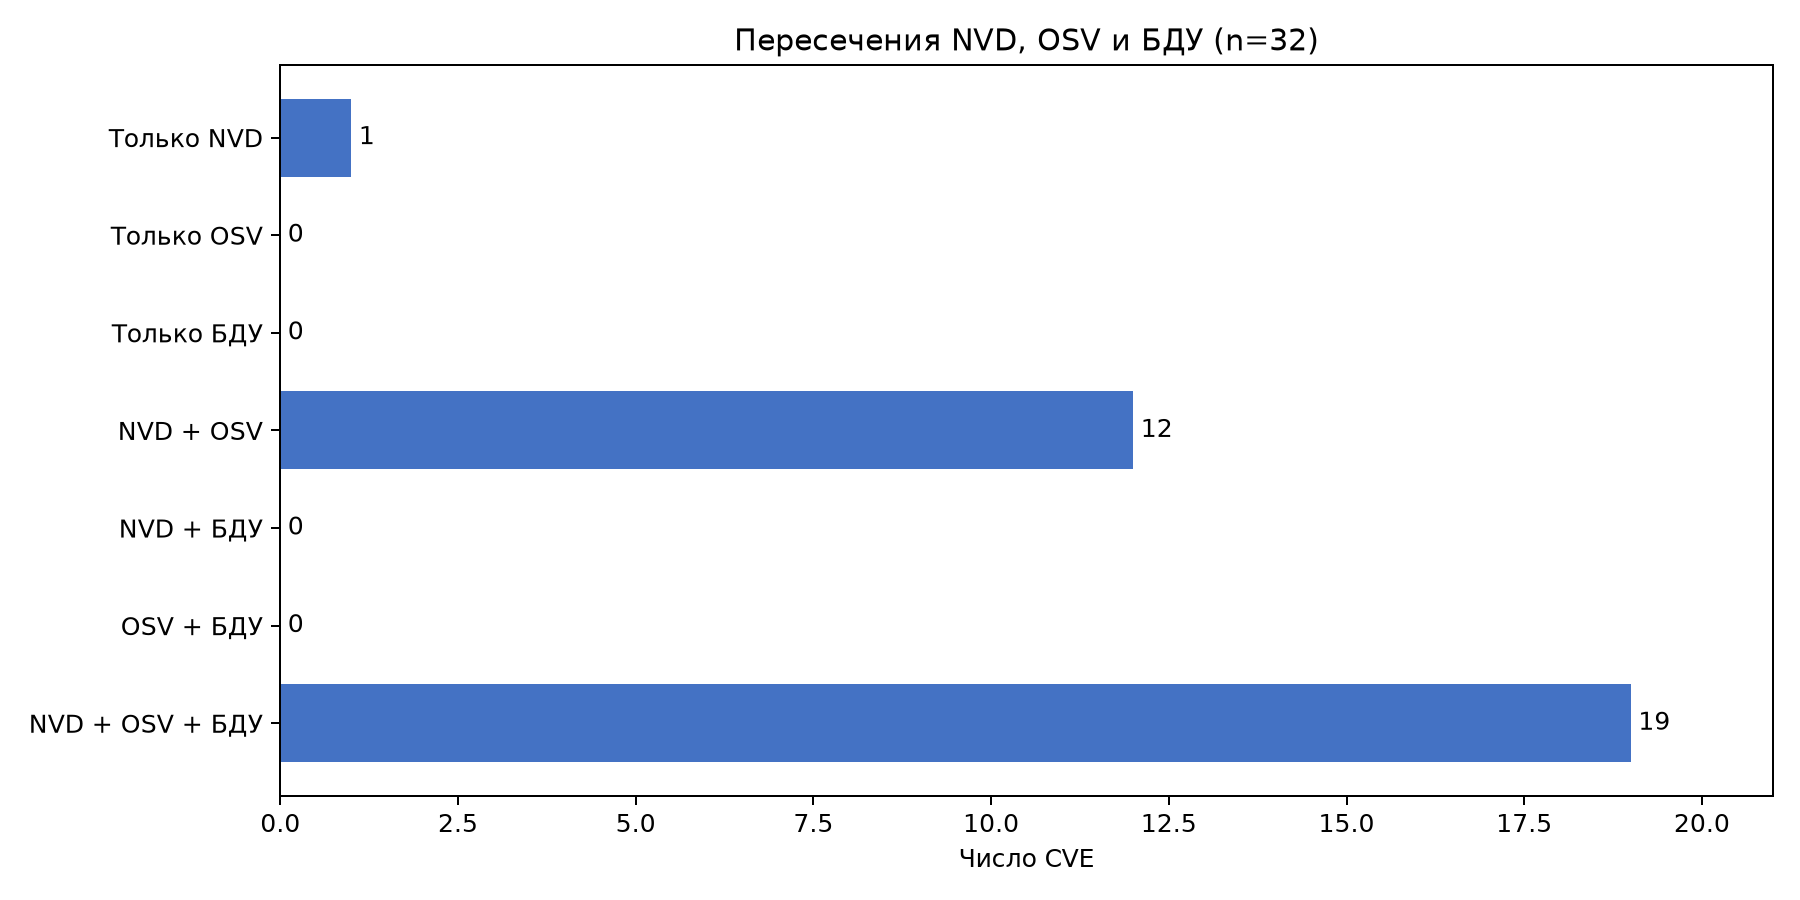
\includegraphics[width=\textwidth]{data/analysis/1_sources/intersections.png}
\caption{Распределение 32 включённых CVE по каталогам; источник: рабочая таблица}
\end{figure}

\begin{table}[ht]
\centering
\caption{Распределение 32 включённых CVE по каталогам}
\begin{tabular}{|l|r|}
\hline
\rowcolor{gray!15}
Каталоги, в которых найдена запись & Число CVE \\
\hline
Только NVD & 1 \\
\hline
NVD и OSV & 12 \\
\hline
NVD, OSV и БДУ & 19 \\
\hline
\end{tabular}
\end{table}

Все 32 включённые CVE присутствуют в NVD; 31 найдена в выборке OSV для пакета \texttt{torch}, а 19 сопоставлены с БДУ. Таким образом, 19 записей есть во всех трёх базах, 12 - в NVD и OSV, одна - только в NVD. Разница в покрытии может быть связана с тем, что NVD получает опубликованные CVE независимо от завершения их анализа NIST, OSV отбирает записи по связи с конкретным пакетом PyPI, а БДУ ведёт отдельный перечень \cite{nvdgeneral,osvdata,bdu}.

Например, CVE-2025-4287 есть в NVD без CPE и не найдена в использованных выборках OSV и БДУ. У CVE-2025-2148 и CVE-2025-2149 совпадают дата публикации и CNA, однако БДУ сопоставлена только со второй. Это показывает, что различие в покрытии нельзя объяснить одним лишь возрастом записи: возможно, на результат повлияли сведения о конкретной CVE и порядок обработки записей в каталогах.

Для 19 совпадающих записей медиана интервала от публикации CVE до включения в БДУ составляет 19 дней. У 16 записей он равен 3--25 дням, а у трёх - 145, 160 и 655 дням. Критичность сама по себе не объясняет разброс: CVE-2025-32434 с оценкой БДУ 9,8 включена через 6 дней, а CVE-2022-45907 с той же оценкой - через 655 дней. Среди восьми записей с высоким уровнем медиана составляет 19 дней, среди восьми со средним - 25 дней.

Возможная причина разброса - разные сроки поступления и обработки сведений в БДУ. Быстрое включение новых CVE и позднее включение отдельных записей прошлых лет могли зависеть от периодической проверки сведений о применяемом ПО; по мере распространения ИИ-сервисов внимание к ML-библиотекам также могло измениться. О групповой обработке говорит совпадение дат: семь CVE, опубликованных 25.09.2025, добавлены в БДУ 14.10.2025, ещё пять с той же датой публикации - 20.10.2025. Такая картина совместима с обработкой общего бюллетеня или тематической проверкой продукта \cite{bdu}.

Полная таблица разниц по каждой из 19 CVE находится в \path{bdu_lag.csv}; числа в этом разделе вычислены по ней и по включённым строкам \workingref.

\section{Частые классы ошибок}

\begin{figure}[htbp]
\centering
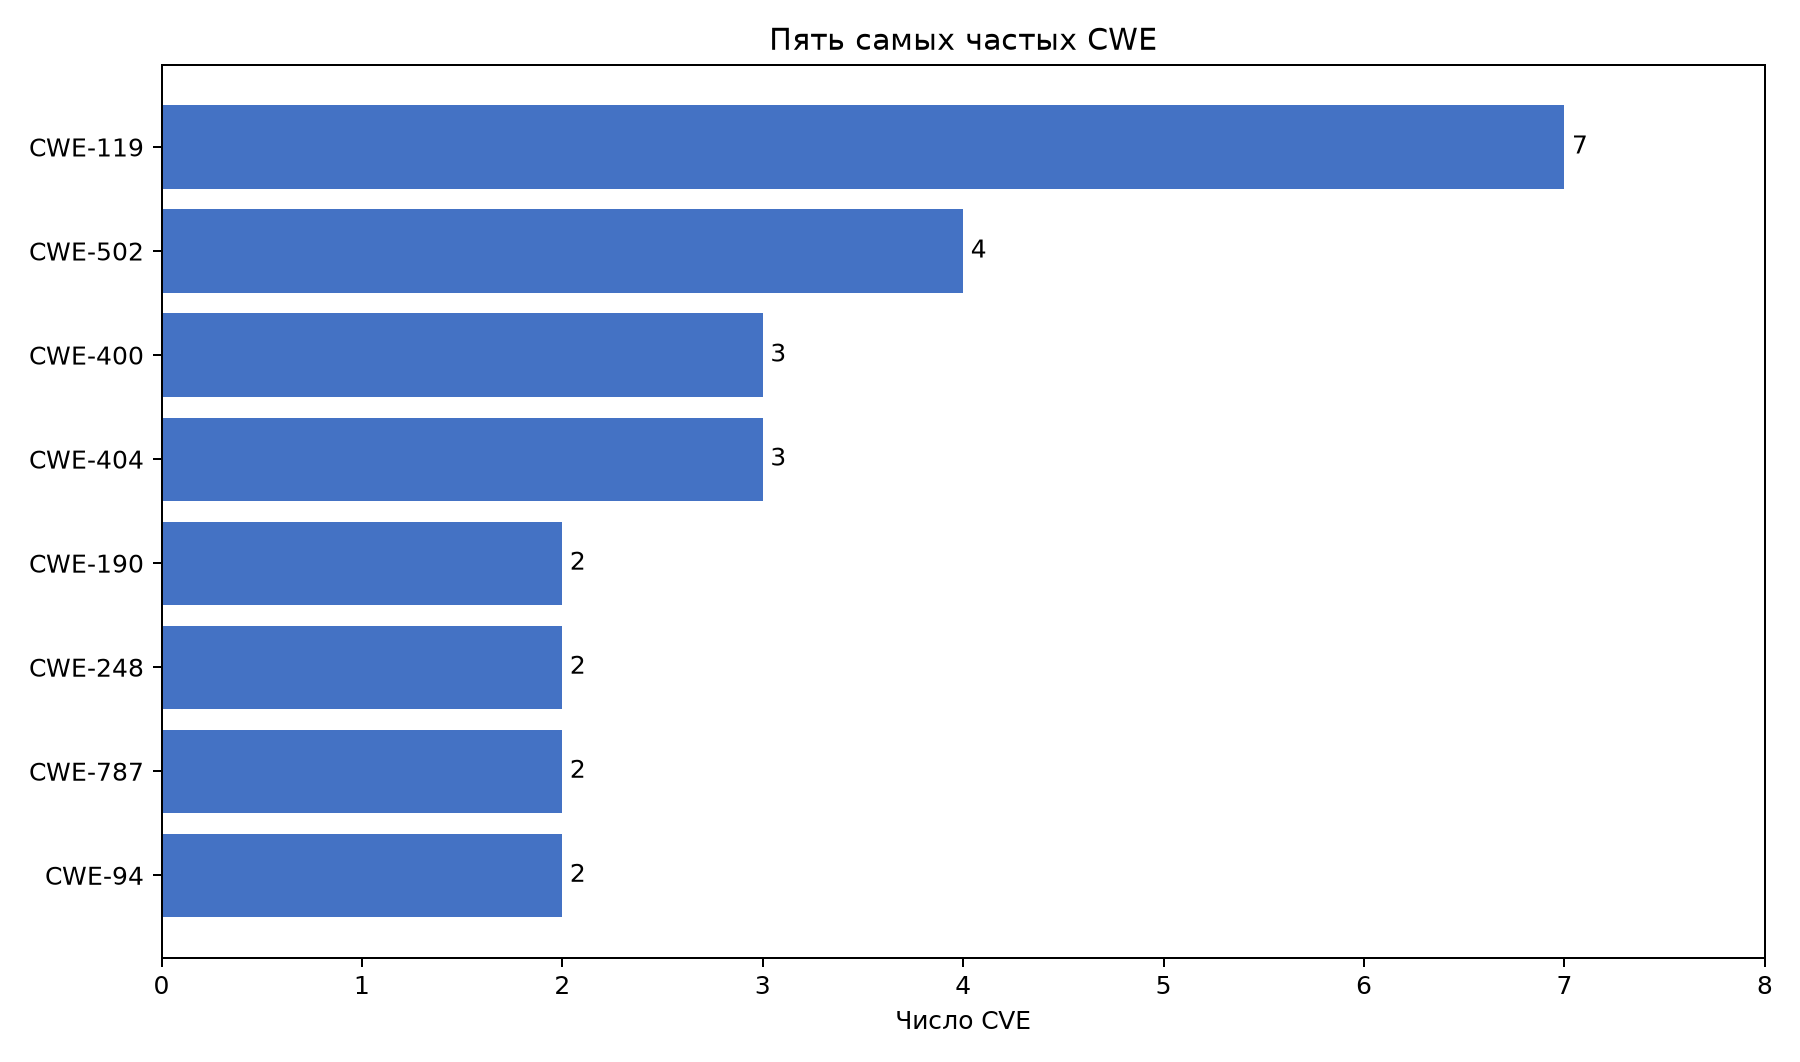
\includegraphics[width=0.94\textwidth]{data/analysis/2_cwe/top_cwe.png}
\caption{Наиболее частые CWE; источник: итоговая таблица}
\end{figure}

\begin{figure}[htbp]
\centering
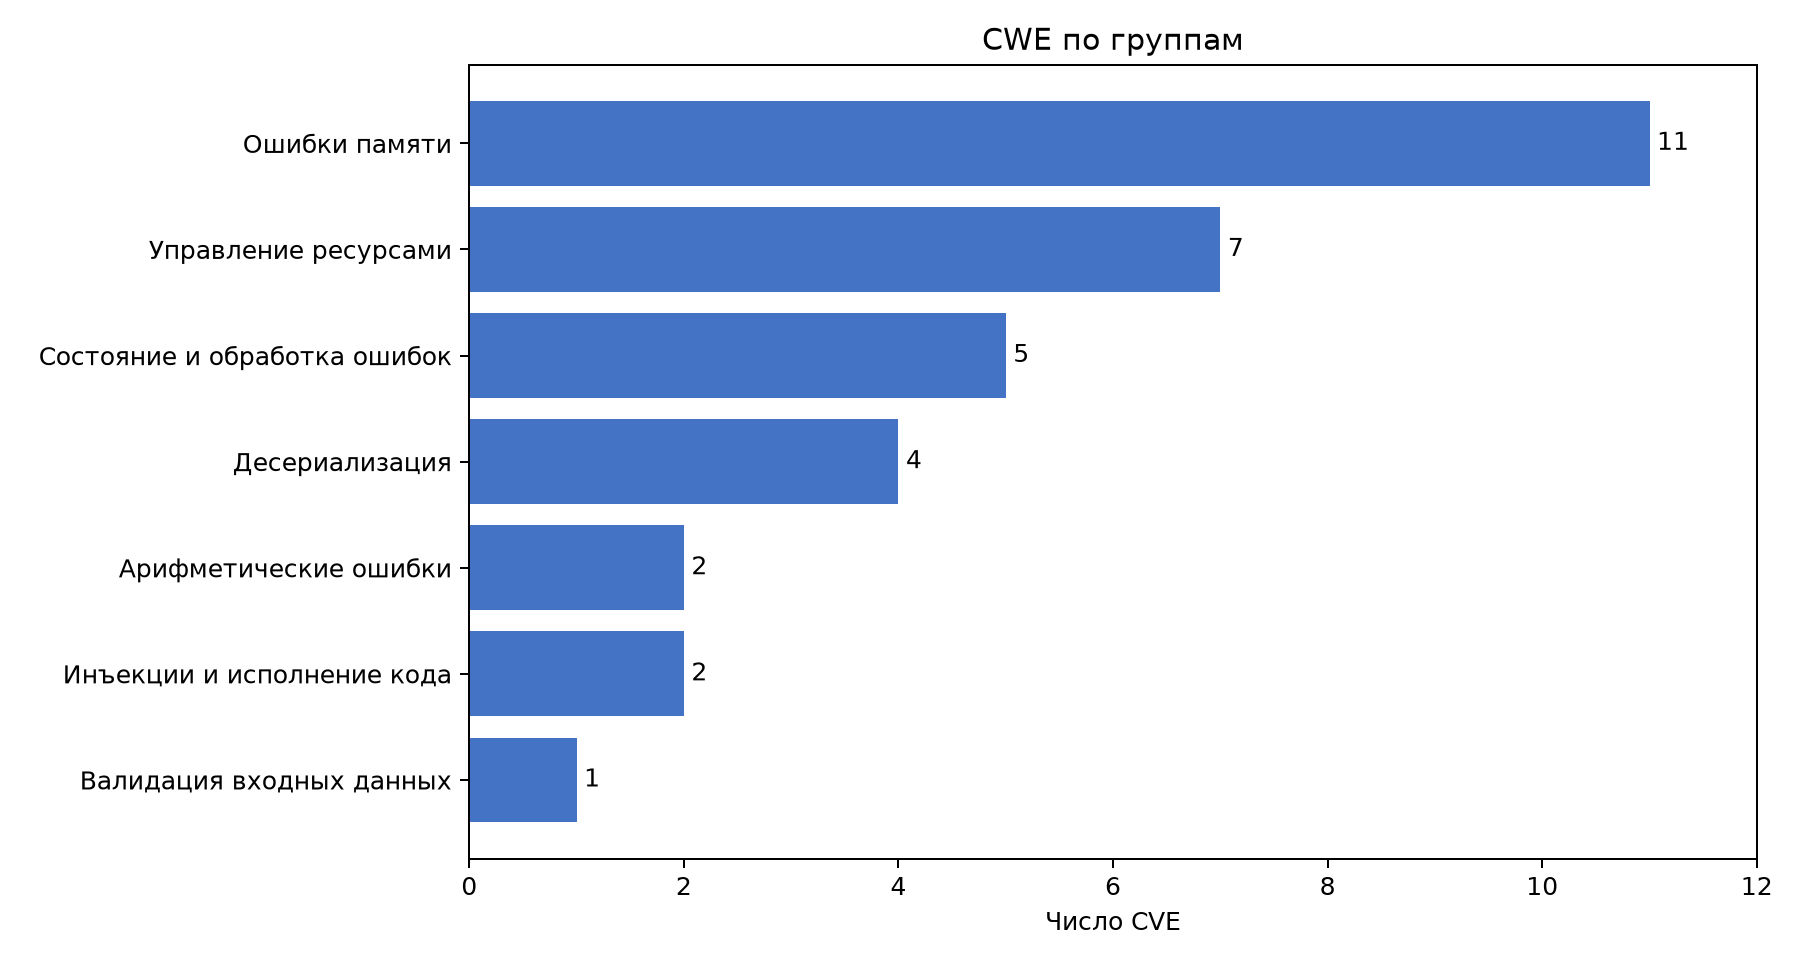
\includegraphics[width=0.94\textwidth]{data/analysis/2_cwe/cwe_groups.png}
\caption{Группы ошибок; одна CVE может входить в несколько групп}
\end{figure}

\begin{table}[ht]
\centering
\caption{Наиболее частые CWE; пятое место разделено}
\begin{tabular}{|l|r|l|}
\hline
\rowcolor{gray!15}
CWE & Число CVE & Место в CWE Top 25 (2025) \\
\hline
CWE-119 & 7 & - \\
\hline
CWE-502 & 4 & 15 \\
\hline
CWE-400 & 3 & - \\
\hline
CWE-404 & 3 & - \\
\hline
CWE-190, 248, 787, 94 & по 2 & 787: 5; 94: 10 \\
\hline
\end{tabular}
\end{table}

При группировке лидируют ошибки памяти (11 CVE), управление ресурсами (7 CVE) и состояние и обработка ошибок (5 CVE). Группы пересекаются: одна CVE может иметь несколько CWE. У пяти CVE указано более одного CWE, у двух код не указан. Разные коды могут отражать неодинаковую детализацию или акцент на разных сторонах ошибки; иногда несколько кодов назначил один источник. Например, для CVE-2025-3136 CNA указала широкий CWE-119, а NVD - более узкий CWE-787; оба учитываются при подсчёте кодов, но CVE остаётся одной записью \cite{cwe119,cwe787}.

В выборке встречаются восемь кодов из CWE Top 25 за 2025 год; хотя бы один такой код есть у 10 из 32 CVE. CWE-502, второй по частоте в выборке, занимает в мировом списке 15-е место. Наиболее частый CWE-119 в Top 25 отсутствует, тогда как его более узкие связанные классы CWE-787 и CWE-125 присутствуют. Различие в рангах связано как со спецификой выборки PyTorch, так и с детализацией присвоенных CWE \cite{top25,cwe119}.

Для ошибок памяти полезны проверки границ и размеров буферов, контроль целочисленных переполнений и проверки памяти в CI. Для отказов в обслуживании нужны ограничения размера входных данных, времени и памяти, а также обработка исключений без аварийного завершения. На границе API следует проверять типы, формы и диапазоны тензоров; при загрузке моделей - не десериализовать недоверенные объекты механизмами, способными исполнять код, и применять безопасные режимы и ограниченные форматы.

\section{Оценки CVSS и EPSS}

\begin{figure}[htbp]
\centering
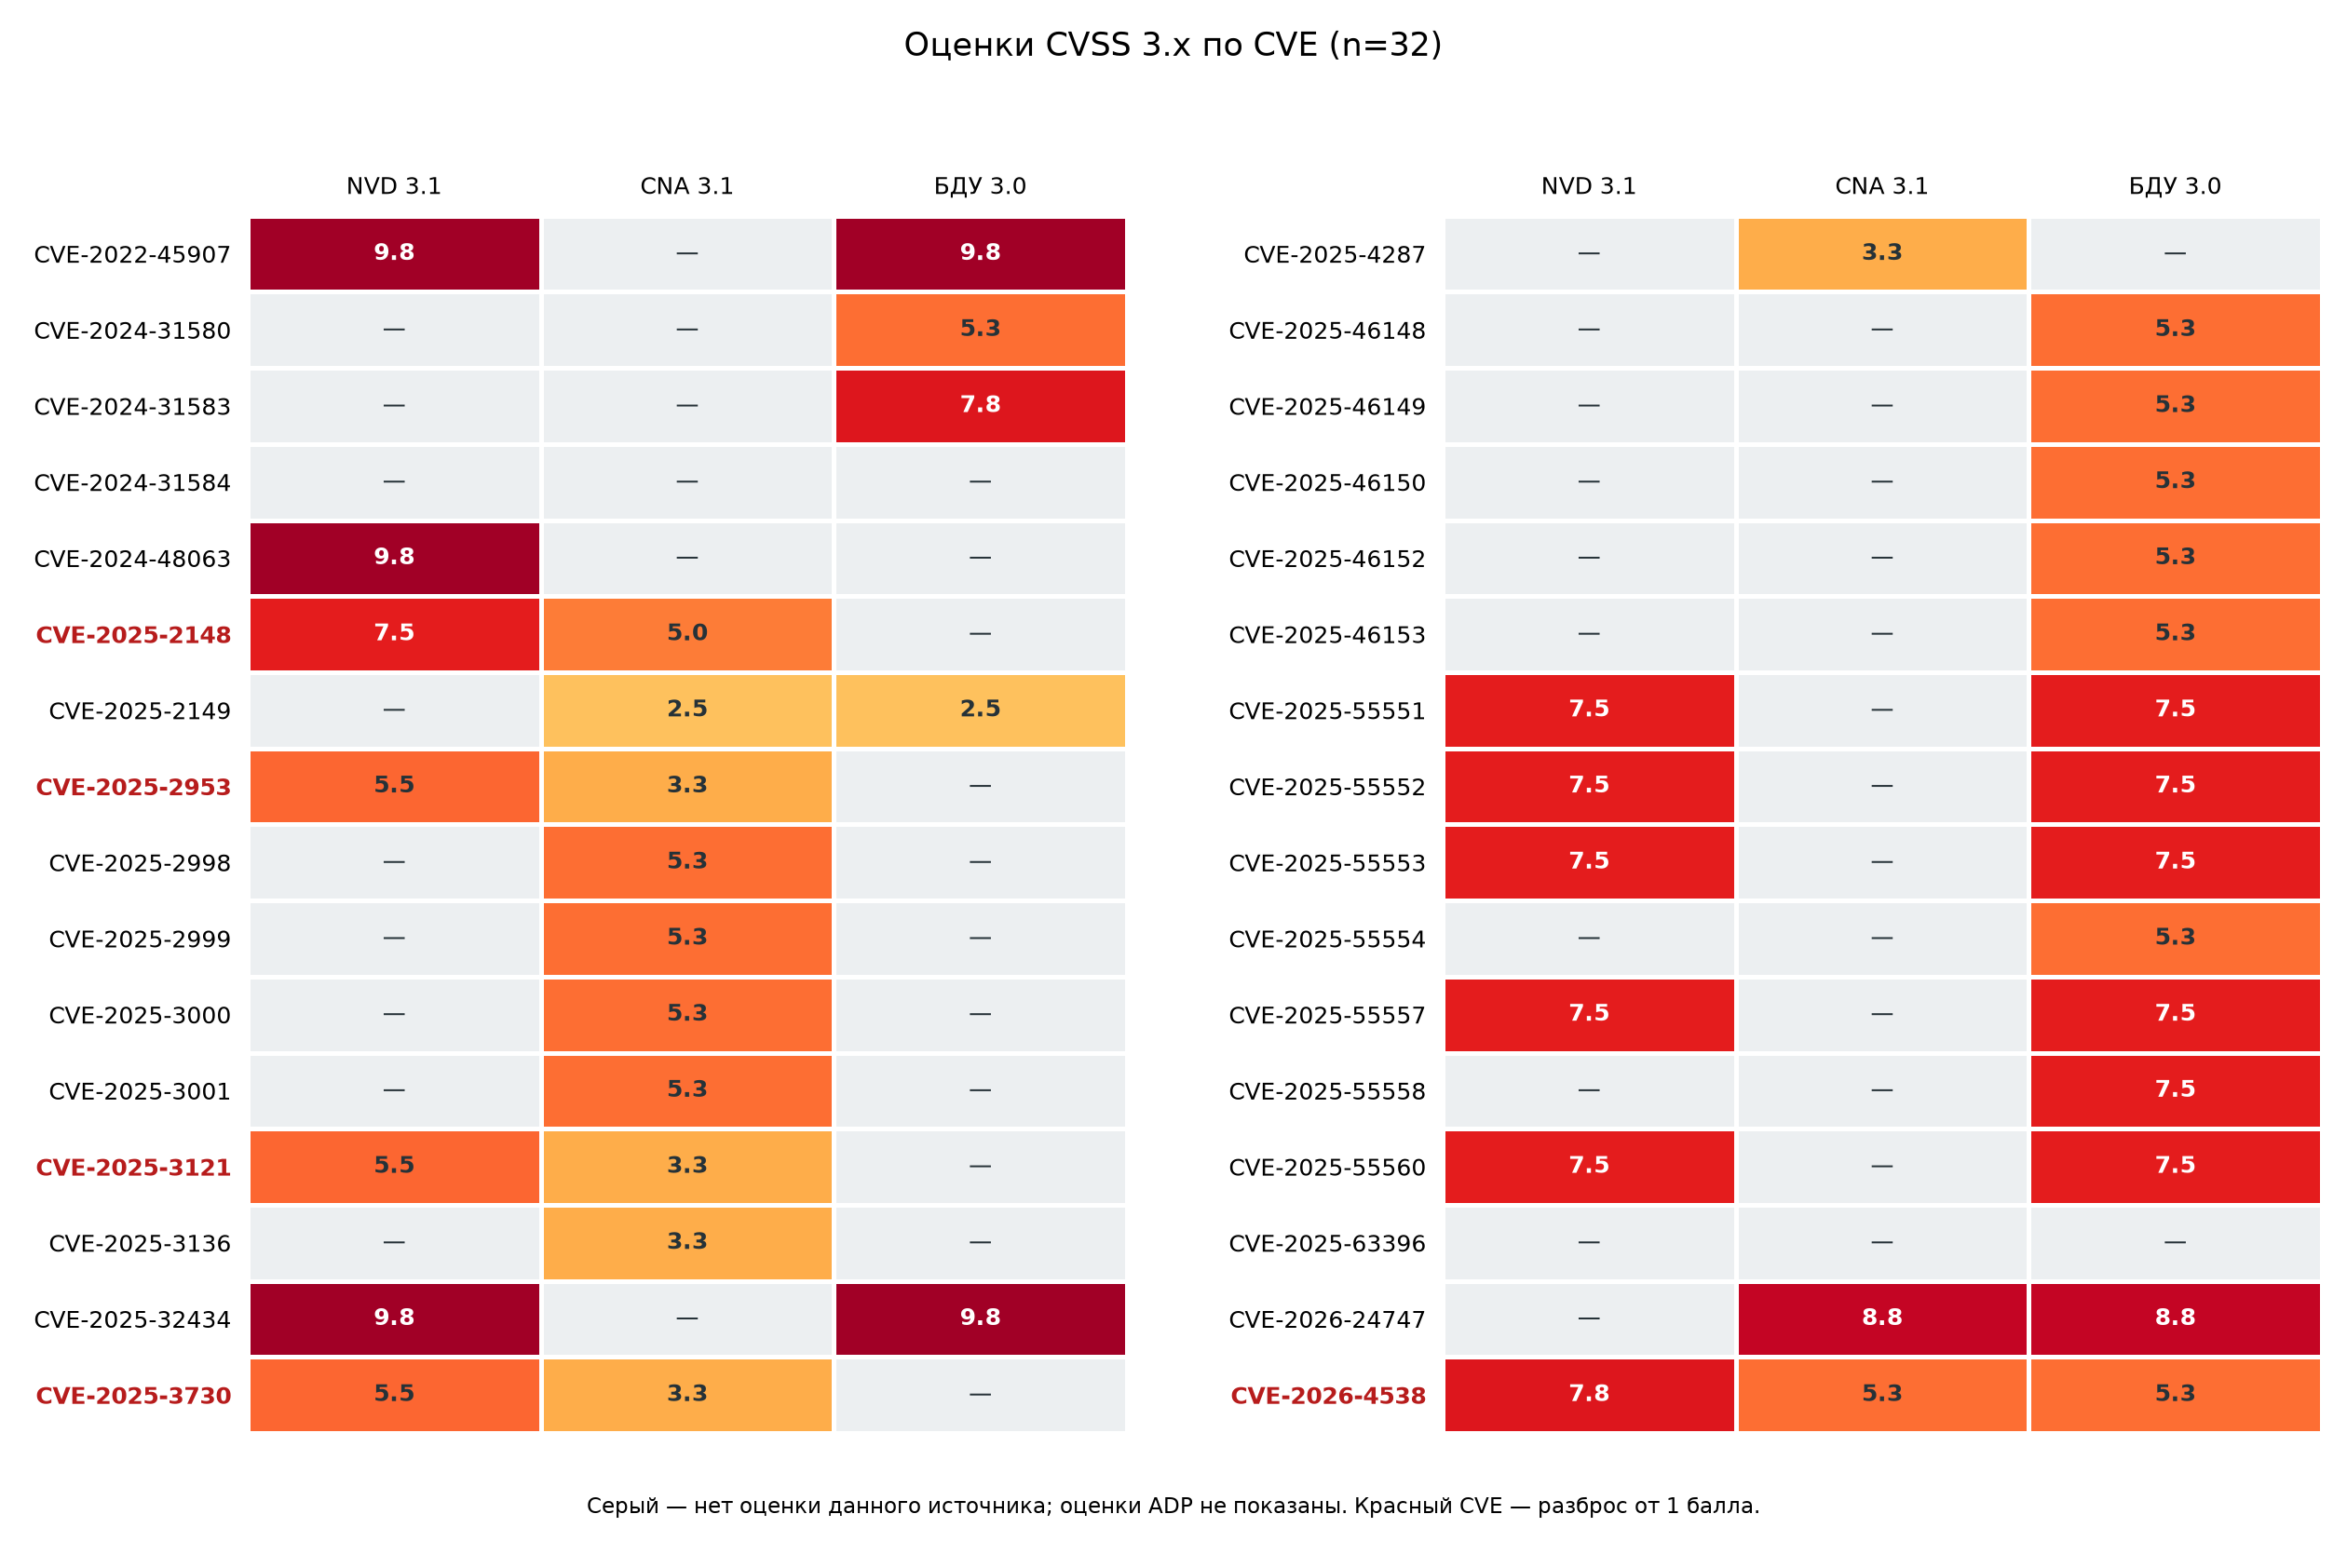
\includegraphics[width=\textwidth]{data/analysis/3_cvss/cvss_by_cve.png}
\caption{Оценки CVSS 3.x для каждой CVE; серые ячейки означают отсутствие оценки выбранного источника}
\end{figure}

\begin{figure}[htbp]
\centering
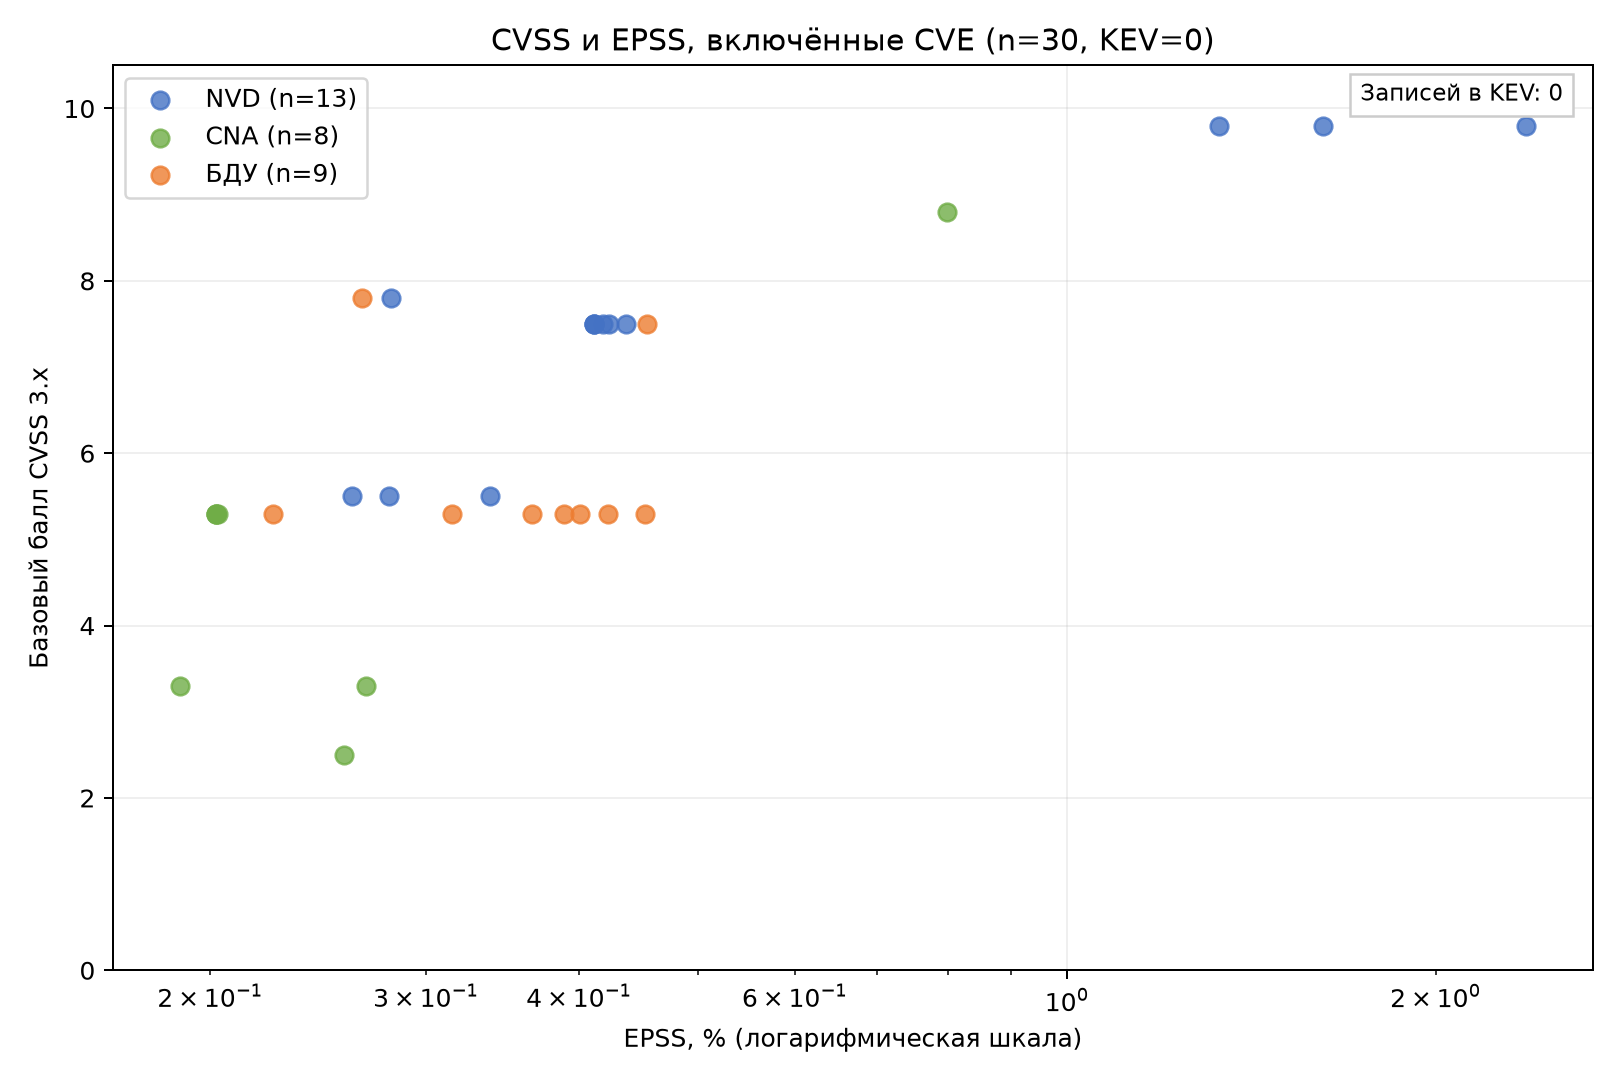
\includegraphics[width=0.86\textwidth]{data/analysis/3_cvss/cvss_epss.png}
\caption{Сопоставление CVSS и EPSS. Записи KEV предусмотрены в легенде, но в этой выборке отсутствуют}
\end{figure}

Сопоставлены 16 пар оценок CVSS 3.x. В шести парах, относящихся к пяти CVE, разница составляет не менее одного балла. В таблице приведены случаи, требующие объяснения по вектору; полный перечень пар находится в \path{comparisons.csv}.

\begin{table}[ht]
\centering
\small
\caption{Расхождения оценок CVSS 3.x не менее одного балла}
\begin{tabular}{|P{3.5cm}|P{4cm}|P{7cm}|}
\hline
\rowcolor{gray!15}
CVE & Баллы по источникам & Отличающиеся метрики по источникам \\
\hline
CVE-2025-2148 & NVD: 7,5; CNA: 5,0 & NVD: C:H/I:H/A:H; CNA: C:L/I:L/A:L \\
\hline
CVE-2025-2953 & NVD: 5,5; CNA: 3,3 & NVD: A:H; CNA: A:L \\
\hline
CVE-2025-3121 & NVD: 5,5; CNA: 3,3 & NVD: A:H; CNA: A:L \\
\hline
CVE-2025-3730 & NVD: 5,5; CNA: 3,3 & NVD: A:H; CNA: A:L \\
\hline
CVE-2026-4538 & NVD: 7,8; CNA: 5,3; БДУ: 5,3 & NVD: C:H/I:H/A:H; CNA: C:L/I:L/A:L; БДУ: C:L/I:L/A:L \\
\hline
\end{tabular}
\end{table}

Во всех пяти CVE из таблицы NVD оценила воздействие выше, чем CNA: для трёх записей сильнее оценено влияние на доступность, для двух - на конфиденциальность, целостность и доступность. Возможная причина - разная полнота сведений на момент оценки или разная трактовка сценария атаки. NVD поясняет, что использует публично доступные материалы на момент анализа, не копирует сторонние векторы и часто расходится с ними, когда сведения об уязвимости недостаточно подробны \cite{nvdscorefaq}.

CNA публикует запись CVE и может назначить собственный балл CVSS. ADP дополняет опубликованную запись отдельными сведениями, не заменяя оценку CNA. Так, у CVE-2024-31584 есть балл 5,5 от CISA-ADP, но нет балла NIST, CNA и БДУ; поэтому сравниваемые ячейки пусты, хотя оценка CVSS у записи существует. В выгрузке БДУ столбец обозначен CVSS 3.0, тогда как на портале для отдельных записей видна метка 3.1. В таблице сохранена версия, указанная в выгрузке; возможные причины различия меток - особенности переноса данных или формата экспорта. Записей из CISA KEV в выборке нет \cite{nvd,kev,bdu}.

\section{Сообщения об уязвимостях и сроки исправления}

\begin{figure}[htbp]
\centering
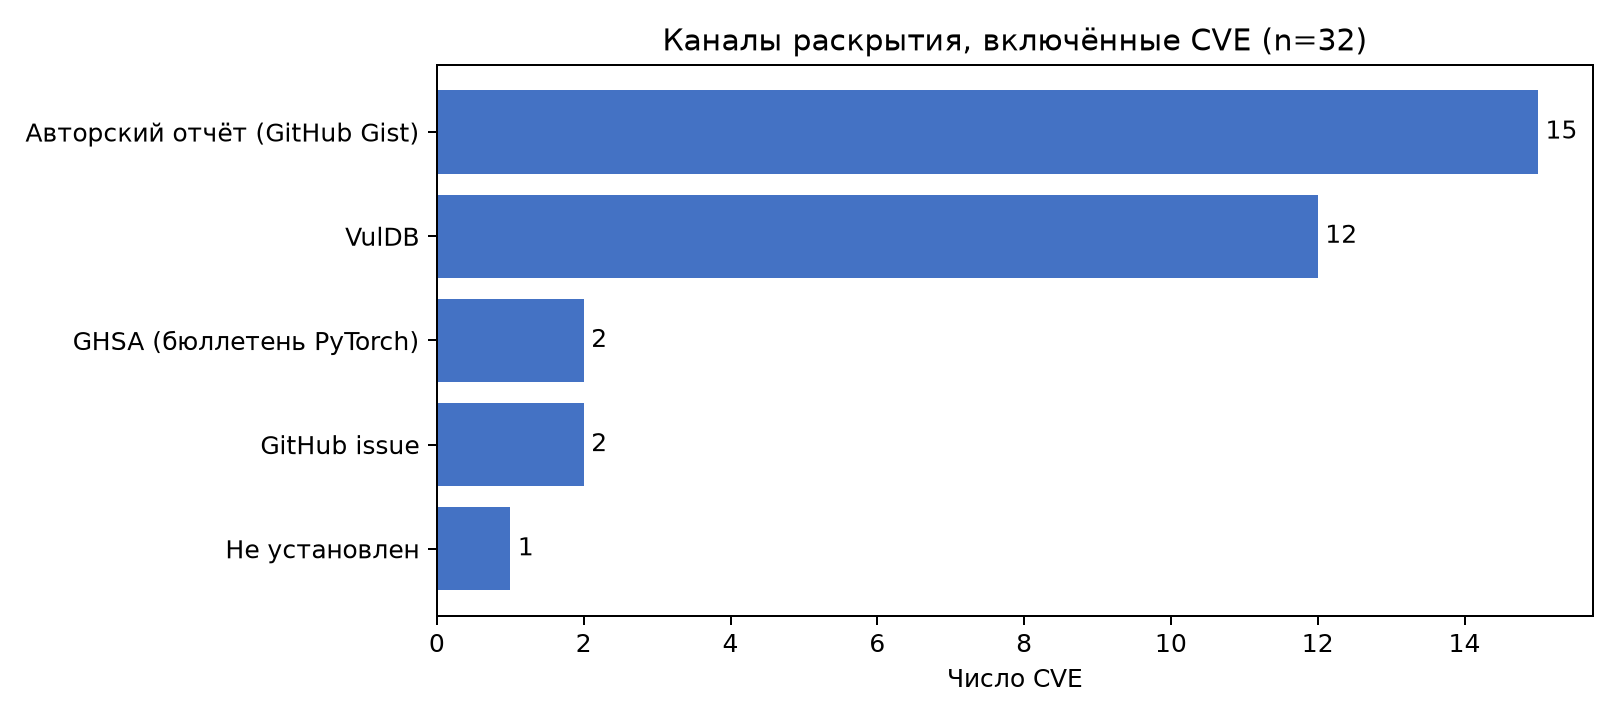
\includegraphics[width=0.9\textwidth]{data/analysis/4_disclosure/channels.png}
\caption{Выбранный публичный канал сообщения для 32 CVE; источник: итоговая таблица}
\end{figure}

\begin{table}[ht]
\centering
\caption{Выбранный публичный канал сообщения для 32 CVE}
\begin{tabular}{|l|r|}
\hline
\rowcolor{gray!15}
Канал & Число CVE \\
\hline
Авторский отчёт на GitHub Gist & 15 \\
\hline
VulDB & 12 \\
\hline
Бюллетень GHSA PyTorch & 2 \\
\hline
GitHub issue & 2 \\
\hline
Не установлен & 1 \\
\hline
\end{tabular}
\end{table}

Для каждой CVE выбран один публичный канал. Преобладают авторские отчёты и заявки вне бюллетеней разработчика; 12 CVE связаны с отчётами одного автора, Shaoyu Yang. Каналом считалась площадка отдельного отчёта об уязвимости: бюллетень, принятая заявка в VulDB или авторская публикация; если отдельного отчёта нет - исходное сообщение в GitHub issue. Например, для CVE, о которых сообщил Shaoyu Yang, учитывались его отдельные отчёты в Gist, хотя им предшествовали GitHub issues. Поле \texttt{reporter} заполнялось по явному указанию исследователя в благодарностях, записи CNA или исходном сообщении; авторство коммита само по себе для этого недостаточно.

Среди 23 записей с подтверждённым исправленным релизом медиана числа дней от выпуска исправления до публикации CVE составляет 50 дней. У 14 CVE выпуск предшествовал публикации, у девяти вышел позже; ещё для девяти дата исправленного релиза не установлена. Например, CVE-2022-45907 опубликована 26.11.2022, а исправленная версия вышла 15.12.2022 (19 дней); для CVE-2025-2953 интервал составил 66 дней, а для CVE-2025-2998 и CVE-2025-2999 - 296 дней \cite{pypi}.

Подробная таблица исследователей, каналов и дат для всех 32 CVE сохранена в \path{disclosure_by_cve.csv}. Поле \texttt{fix\_date} здесь означает дату выхода первой подтверждённой исправленной стабильной версии пакета \texttt{torch} на PyPI. Дата самого коммита фиксируется отдельно и не заменяет дату доступного пользователю релиза.

\section{Подробный разбор CVE-2026-24747}

\subsection{Условия и последствия}

Бюллетень PyTorch относит к уязвимым версии не новее 2.9.1 и называет 2.10.0 первой исправленной версией. Атакующий должен добиться загрузки подготовленного им checkpoint процессом с уязвимой версией PyTorch через \verb|torch.load(..., weights_only=True)|. Разработчик описывает два недостатка проверки: операции pickle \texttt{SETITEM}/\texttt{SETITEMS} применялись к объектам, не являющимся словарями, и число элементов хранилища не сопоставлялось с фактическим размером записи архива. Возможны повреждение памяти и, по оценке PyTorch, выполнение произвольного кода в процессе жертвы. В этой работе возможность RCE не проверялась \cite{ghsa}.

\subsection{Исправление в коде}

В PR \#170085 добавлена проверка типа объекта перед выполнением \texttt{SETITEM} и \texttt{SETITEMS}. До исправления после снятия ключа и значения со стека выполнялась запись \verb|self.stack[-1][k] = v|; после исправления ей предшествует вызов \verb|self._check_set_item_target("SETITEM")|. Новая функция допускает точные типы \texttt{dict}, \texttt{OrderedDict} и \texttt{Counter}, иначе поднимает \texttt{UnpicklingError}. Во второй части исправления C++ код проверяет равенство фактического размера записи и \verb|numel * elementSize(scalar_type)| до создания хранилища. PR содержит регрессионные проверки для обеих ситуаций; коммит \texttt{0e2459f} перенёс изменения в ветку 2.10.0 \cite{fixpr,fixcommit,release}.

Опубликованная запись CVE содержит ссылки на issue \#163105 и коммит \texttt{954dc5183ee9205cbe79876ad05dd2d9ae752139}. Они относятся к сериализации состояния планировщика SWALR и не подтверждают исправление CVE-2026-24747. Для данного разбора использованы PR \#170085 и коммит переноса \texttt{0e2459f} \cite{wrongcommit,fixpr}.

\subsection{Связь классификаций и наблюдение}

\begingroup
\clubpenalty=10000
\widowpenalty=10000

Сопоставление классификаций строится от слабости в коде к способу её использования, а затем к сценарию атаки. При загрузке checkpoint PyTorch обрабатывает недоверенные сериализованные данные и недостаточно проверяет типы объектов и размеры хранилища. Этому механизму соответствует \textbf{CWE-502} (Deserialization of Untrusted Data). Указанный в записи CNA дополнительный класс CWE-94 учитывается, но основная цепочка строится на CWE-502, поскольку он непосредственно описывает проблему десериализации \cite{cwe502,fixpr}.

Когда атакующий помещает некорректное содержимое в сериализованный объект и добивается его обработки приложением, способ атаки описывается шаблоном \textbf{\mbox{CAPEC-586} - Object Injection}. В рассматриваемой CVE таким объектом служит специально подготовленный checkpoint: его разбор может вызвать повреждение памяти и привести к выполнению произвольного кода. Связь CWE-502 $\rightarrow$ CAPEC-586 явно представлена в каталоге MITRE \cite{capec586,ghsa}.

ATLAS позволяет описать доставку и использование такого файла в жизненном цикле модели. Если атакующий распространяет вредоносный checkpoint через репозиторий моделей, откуда его получает целевая система, этому этапу соответствует \textbf{AML.T0010.003 - Supply Chain Compromise: Model Repository}. Шаблон описывает попадание вредоносной модели в цепочку поставок; последующая загрузка может выполняться исследователем вручную или автоматически в ML-пайплайне \cite{atlas202610}.

Когда исследователь или оператор инициирует загрузку подготовленного checkpoint, пользовательское действие описывается \textbf{AML.T0011.000 - User Execution: Unsafe AI Artifacts}. Файл модели выступает небезопасным ИИ-артефактом, обработка которого запускает эксплуатацию ошибки загрузчика. Этот вариант выбран основным для пользовательского сценария из бюллетеня PyTorch. Если файл ранее получен через репозиторий, AML.T0010.003 и AML.T0011.000 описывают последовательные этапы одной атаки: доставку модели и её загрузку \cite{atlas202610,ghsa}.

ATT\&CK позволяет рассмотреть эксплуатацию с точки зрения приложения, в котором обрабатывается файл, и точки входа в систему \cite{ctidmapping}. Если исследователь загружает checkpoint в клиентском приложении на своей рабочей станции и ошибка загрузчика позволяет выполнить произвольный код, подходит \textbf{T1203 - Exploitation for Client Execution}. Здесь CAPEC-586 описывает способ воздействия через сериализованный объект, а T1203 - эксплуатацию уязвимости клиентского приложения \cite{attack1203}.

В случае если входом служит доступный из Интернета сервис, который принимает checkpoint и передаёт его уязвимому загрузчику, для описания первоначального доступа подходит \textbf{T1190 - Exploit Public-Facing Application}. Атакующий использует обработку файла на стороне сервера, чтобы получить доступ в контексте его рабочего процесса. Выбор этой техники определяется публичной точкой входа и ролью эксплуатации в получении доступа \cite{attack1190}.

Общая связь CWE-502 $\rightarrow$ CAPEC-586 раскрывается через условия конкретного сценария. ATLAS отражает путь модельного артефакта до загрузки, а ATT\&CK - эксплуатацию клиентского приложения или публичного сервиса. Соответствия CAPEC с этими техниками установлены при анализе сценариев данной работы. Все пять перечисленных шаблонов атак представлены объектами \texttt{attack-pattern} в STIX 2.1; их связи с уязвимостью и мерой защиты сохранены в файле \stixref, который формируется скриптом \path{__main__.py} при помощи библиотеки \texttt{stix2}.

Для наблюдения за таким сценарием следует сопоставлять событие загрузки checkpoint с последующими ошибками и поведением процесса. В исправленной версии попытка обработки некорректного файла может сопровождаться сообщениями \texttt{Can only SETITEM...} или \texttt{record size ... does not match expected size}, если приложение журналирует исключения. В уязвимой версии аварийное завершение процесса, необычный дочерний процесс или исходящее соединение сразу после загрузки служат поводом для расследования, но не доказывают эксплуатацию этой CVE. Публичный бюллетень не содержит уникального набора индикаторов компрометации \cite{fixcommit,ghsa}.

\endgroup

\section{Модель угроз для сервиса загрузки моделей}

\subsection{Типовой сервис и его пользователи}

В работе рассмотрена учебная модель корпоративного ИИ-сервиса на PyTorch. Сервис предназначен для загрузки, дообучения и публикации моделей, полученных от исследователей или из внешних репозиториев. Исследователь передаёт файл контрольной точки модели (checkpoint) через веб-интерфейс. Инженером машинного обучения проверяется полученный артефакт и запускается дообучение, после которого оператор принимает решение о публикации. Пользователям и прикладным системам предоставляется API инференса. Инфраструктура обслуживается администратором, события мониторинга поступают специалисту по безопасности.

Загруженный файл сначала помещается в карантинное хранилище сервиса. Затем отдельным процессом PyTorch проверяется его содержимое и подготавливается модель для дообучения. После согласования результат переносится в реестр разрешённых моделей и передаётся рабочим процессам инференса. В состав сервиса также входят очередь заданий, хранилище обучающих данных, средства управления секретами и журнал событий. Внешние репозитории и сеть провайдера находятся за пределами доверенной инфраструктуры организации.

Защите подлежат закрытые датасеты, веса собственных моделей, запросы клиентов и служебные токены. Требуется также обеспечить доступность вычислений для легальных пользователей. Границы доверия проходят между внешним файлом и загрузчиком, загрузчиком и хранилищами, проектами разных пользователей, реестром моделей и продуктивной средой. Одобрение файла оператором само по себе не подтверждает безопасность содержимого. Проверка требуется при каждом переходе артефакта через соответствующую границу.

При оценке исходного риска приняты следующие условия: процесс загрузки использует PyTorch версии не новее 2.9.1, читает данные проекта и устанавливает исходящие соединения. В защищённом варианте внешний checkpoint проверяется в отдельной среде до предоставления доступа к закрытым данным. Для системы, принимающей только проверенные внутренние артефакты, применимость рассматриваемого сценария оценивается с учётом фактических каналов поступления моделей.

Возможными последствиями атаки являются простой сервиса, срыв сроков обработки, раскрытие датасетов и весов, подмена модели и получение недостоверных результатов. Для организации возникают расходы на восстановление и риск утраты коммерческой тайны.

\subsection{Выбор угроз БДУ и обоснование актуальности}

Согласно Методике ФСТЭК от 05.02.2021, при оценке угроз устанавливаются нарушитель, объект воздействия, доступный интерфейс, способ реализации и возможные последствия. Актуальность определяется наличием осуществимого сценария в рассматриваемой системе \cite{fstekmethod}. В выбранной архитектуре такой сценарий возникает при передаче внешнего файла загрузчику.

При оценке по \href{https://bdu.fstec.ru/threat}{классическому перечню угроз БДУ ФСТЭК} для рассматриваемого сервиса выбраны УБИ.006, УБИ.033, УБИ.192 и УБИ.088. Условия их реализации приведены в таблице~\ref{tab:step5-threats}. Предполагается, что нарушителем контролируется содержимое внешнего файла модели. Для последующего копирования закрытых данных дополнительно необходимы выполнение кода и достаточные права скомпрометированного процесса \cite{bduthrlist}.

\begingroup\small
\begin{longtable}{|P{4.3cm}|P{6.0cm}|P{3.5cm}|}
\caption{Угрозы классического перечня и условия их реализации}\label{tab:step5-threats}\\
\hline
\rowcolor{gray!15}
УБИ и точное название & Объект, способ и условие реализации & Последствия \\
\hline
\endfirsthead
\hline
\rowcolor{gray!15}
УБИ и точное название & Объект, способ и условие реализации & Последствия \\
\hline
\endhead
\href{https://bdu.fstec.ru/threat/ubi.006}{УБИ.006}\newline Угроза внедрения кода или данных & Воздействие направлено на прикладное ПО загрузчика. Переданный нарушителем checkpoint обрабатывается после импорта инженером. Ошибки проверки сериализованных объектов создают возможность воздействия на процесс PyTorch. & Внедрение кода или данных может нарушить конфиденциальность, целостность и доступность в пределах прав процесса. \\
\hline
\href{https://bdu.fstec.ru/threat/ubi.033}{УБИ.033}\newline Угроза использования слабостей кодирования входных данных & Объектом выступает прикладное ПО, принимающее файл. Нарушителем задаются структура checkpoint, типы объектов и метаданные хранилища. Уязвимым загрузчиком недостаточно проверяется их согласованность. & Возможны повреждение памяти, сбой процесса, нарушение целостности и доступности. \\
\hline
\href{https://bdu.fstec.ru/threat/ubi.192}{УБИ.192}\newline Угроза использования уязвимых версий программного обеспечения & Используется библиотека PyTorch версии $\leq 2.9.1$. При допуске внешних моделей к обработке не учитывается опубликованная уязвимость CVE-2026-24747. & Эксплуатация известной уязвимости может привести к RCE, утечке, изменению данных или отказу процесса. \\
\hline
\href{https://bdu.fstec.ru/threat/ubi.088}{УБИ.088}\newline Угроза несанкционированного копирования защищаемой информации & Защищаемыми объектами являются файлы датасетов и закрытых весов. После успешного RCE читаются доступные процессу незашифрованные данные, копия которых передаётся наружу. Необходимы избыточные права и доступный канал вывода. & Нарушается конфиденциальность данных и модели. Изоляция загрузчика и запрет доступа к этим ресурсам прерывают рассматриваемую цепочку. \\
\hline
\end{longtable}
\endgroup

УБИ.006, УБИ.033 и УБИ.192 характеризуют разные аспекты одной атаки. При оценке риска учитывается их связь в общей последовательности действий. УБИ.088 описывает возможное развитие сценария после получения доступа к данным. Для рассматриваемого случая CWE-502 непосредственно отражает проблему обработки недоверенных сериализованных данных: само расширение \texttt{.pth} не определяет поведение файла при загрузке.

При оценке по \href{https://bdu.fstec.ru/threat-section/threats}{новому перечню угроз БДУ ФСТЭК} для того же сценария выбраны УБИ.1 «Угроза утечки информации», УБИ.2 «Угроза несанкционированного доступа», УБИ.6 «Угроза отказа в обслуживании», УБИ.8 «Угроза нарушения функционирования (работоспособности)» и УБИ.9 «Угроза получения информационных ресурсов из недоверенного или скомпрометированного источника» \cite{bduubi}.

Для рассматриваемого сценария в матрице нового перечня учитываются связи с пятью выбранными угрозами. С сервером О.2 и устройством хранения данных О.4 связаны УБИ.1, УБИ.2, УБИ.6 и УБИ.8. Для УБИ.9 указан объект О.11 «Информация (данные), содержащаяся в системах и сетях». В сценарии этому объекту соответствует содержимое файла модели, поступающего из внешнего источника \cite{bduubi}.

Способ СП.1.1 «Эксплуатация известных уязвимостей» связан с выбранными УБИ.1, УБИ.2, УБИ.6 и УБИ.8. Для СП.2.1 «Использование недостатков, связанных с неполнотой проверки вводимых (входных) данных» отмечены связи со всеми пятью выбранными угрозами. Отказ при обработке некорректного checkpoint в этой схеме учитывается через УБИ.6 и УБИ.8 \cite{bduubi}.

В профильном разделе БДУ \href{https://bdu.fstec.ru/threat/ai}{«Угрозы ИИ»} импорт и дообучение модели относятся к инфраструктуре разработчика. Основным способом для выбранного сценария является СП.1, предусматривающий эксплуатацию недостатков ПО, включая фреймворки машинного обучения. Способ СП.2 дополнительно учитывается при наличии опасного компонента или недекларированной возможности во входной модели. Применимость этого способа устанавливается по содержимому артефакта и характеру воздействия. Возможными последствиями являются утечка данных, кража модели и нарушение её функционирования \cite{bduai}.

При дообучении в инфраструктуре оператора дополнительно рассматриваются угрозы, относящиеся к инфраструктуре разработчика. Такое требование приведено в профильном разделе БДУ. Для сервиса, выполняющего только инференс, отдельно оцениваются угрозы инфраструктуры оператора. Указанные выше СП.1 и СП.2 относятся к таблице 1 раздела «Угрозы ИИ». В таблице 2, посвящённой оператору, под этими номерами приведены другие способы воздействия \cite{bduai}.

\subsection{Нарушитель и сценарий атаки}

В модели принят внешний нарушитель со средними возможностями уровня \textbf{Н3}. Предполагается, что он способен исследовать загрузчик и самостоятельно разработать средство эксплуатации, предназначенное для получения закрытых данных проекта. Нарушителем контролируется внешний репозиторий либо публикуемый checkpoint. Первоначальный доступ к учётной записи администратора, датасетам и оборудованию сервера отсутствует. Предложенная модель импортируется инженером организации через легитимный интерфейс.

Выбор Н3 обусловлен допущением о самостоятельной разработке средства атаки. Оценка CVSS и использование языка Python сами по себе не определяют уровень возможностей нарушителя. Применение готовых общедоступных средств могло бы соответствовать уровням Н1--Н2. Наличие такого средства для рассматриваемой CVE в работе не устанавливалось \cite{fstekmethod}.

\begingroup\small
\begin{longtable}{|P{3.4cm}|P{5.8cm}|P{4.6cm}|}
\caption{Сценарий импорта вредоносного checkpoint}\label{tab:step5-scenario}\\
\hline
\rowcolor{gray!15}
Тактики и техники & Действие в рассматриваемом сервисе & Наблюдаемый след и условия \\
\hline
\endfirsthead
\hline
\rowcolor{gray!15}
Тактики и техники & Действие в рассматриваемом сервисе & Наблюдаемый след и условия \\
\hline
\endhead
Т1, Т1.1\newline Сбор информации из публичных источников & Изучаются опубликованные сведения о PyTorch, форматах моделей и порядке их проверки и импорта. & Пассивная разведка может не оставить следов в сервисе. До проверки сведения о версии ПО остаются предположением. \\
\hline
Т2, Т2.5\newline Эксплуатация уязвимостей компонентов систем и сетей\newline Т3, Т3.5\newline Эксплуатация уязвимостей типа RCE & Инженером инициируется загрузка подготовленного checkpoint. При успешной эксплуатации CVE-2026-24747 нарушитель получает возможность выполнять код с правами загрузчика. Т2.5 характеризует первоначальный доступ, Т3.5 отражает исполнение кода в рамках того же эпизода. & Фиксируются источник, хеш файла, пользователь, время импорта и версия загрузчика. Возможны аварийное завершение процесса, необычные дочерние процессы и обращения к файлам. Факт импорта или сбоя сам по себе не подтверждает RCE. \\
\hline
Т10, Т10.1\newline Несанкциониро\-ванный доступ к информации в файловой системе & Вредоносным кодом читаются доступные загрузчику датасеты и веса другого проекта. Нарушается конфиденциальность защищаемых файлов. & Обращения отражаются в аудите доступа к контрольным файлам. Необходимы недостаточная изоляция и фактическая доступность данных. \\
\hline
Т9, Т9.3\newline Вывод информации через разрешённые известные порты внешних серверов & Прочитанные данные передаются на HTTPS-сервер нарушителя через TCP-порт 443, разрешённый правилами межсетевого экрана. & После импорта фиксируется исходящее соединение с внешним сервером. Передача копии защищаемых данных за пределы системы завершает реализацию УБИ.088. Само соединение ещё не подтверждает содержание передачи. \\
\hline
\end{longtable}
\endgroup

В соответствии с пунктом 5.3.4 Методики последовательность действий устанавливается применительно к конкретному сценарию. В рассматриваемой цепочке Т10.1 описывает чтение защищаемых файлов, нарушающее их конфиденциальность. Последующая передача полученной копии соответствует Т9.3. Размещение Т10.1 перед Т9.3 отражает эту причинную связь. Достижение цели по УБИ.088 оценивается по совокупности доступа к данным, их копирования и вывода \cite{fstekmethod}.

Т2.5 и Т3.5 объединены в одной строке, поскольку характеризуют единый эпизод эксплуатации с двумя тактическими задачами. Повышение прав до root, закрепление в системе и выход из контейнера для этой цепочки не требуются. При завершении обработки только сбоем процесса рассматривается ветвь отказа, соответствующая Т10.10. Чтение и вывод данных в этом случае остаются неподтверждёнными.

В классификации MITRE ATLAS получение модели через внешний репозиторий соотнесено с AML.T0010.003. Действию инженера, запускающего обработку небезопасного артефакта, соответствует AML.T0011.000. Для публичного API, самостоятельно принимающего и обрабатывающего checkpoint, первоначальный доступ может описываться техникой ATT\&CK T1190. Техника T1203 применяется к эксплуатации клиентского приложения. \cite{atlas202610,attack1190,attack1203}.

\subsection{Меры защиты и критерии проверки}

Предложенные меры воздействуют на разные этапы рассмотренного сценария. Обновлением PyTorch устраняется известный дефект, контролем артефактов ограничивается поступление неподтверждённых файлов, изоляцией загрузчика сокращается объём доступных ему ресурсов.

\begingroup\small
\begin{longtable}{|P{4.1cm}|P{5.1cm}|P{4.6cm}|}
\caption{Меры защиты, проверки и критерии приёмки}\label{tab:step5-controls}\\
\hline
\rowcolor{gray!15}
Мера и связанные угрозы & Порядок проверки & Критерий успешности \\
\hline
\endfirsthead
\hline
\rowcolor{gray!15}
Мера и связанные угрозы & Порядок проверки & Критерий успешности \\
\hline
\endhead
Обновление PyTorch и проверка зависимостей (УБИ.192, УБИ.033). Первой исправленной версией для данной CVE является 2.10.0. & Сопоставляются версия установленного пакета \texttt{torch}, lock-файл и состав конечного образа по SBOM. Выполняются регрессионные проверки некорректных типов и размеров, предусмотренные исправлением PyTorch. & Используется версия, исправляющая CVE-2026-24747. Некорректные файлы отклоняются контролируемо, допустимая модель загружается. Сохранены отчёты сканера и тестов. \\
\hline
Контроль формата и загрузчика (УБИ.006, УБИ.033). Для весов предпочтителен safetensors. Обработка прежних форматов ограничивается разрешёнными случаями. & Проверяются явные параметры \texttt{weights\_only=True} и \texttt{map\_location="cpu"} при вызове \texttt{torch.load}. Контролируются типы, формы, число и общий объём тензоров. & Неизвестные форматы и объекты отклоняются. Ошибка не вызывает повторной загрузки с \texttt{weights\_only=False}. Проверяется содержимое файла независимо от расширения. \\
\hline
Разделение карантина и реестра, контроль происхождения и неизменности (УБИ.006 и новая УБИ.9). & Проверяются права загрузчика, согласующего и издателя. Предпринимаются попытки подменить одобренный файл, предъявить неизвестную подпись или несовпадающий хеш. & Несогласованная публикация и подмена запрещены. Запускается файл с одобренной контрольной суммой, сверенной по доверенной записи. Сумма от неизвестного отправителя не считается достаточным подтверждением. \\
\hline
Изоляция загрузчика и ограничение прав (УБИ.006, УБИ.088). Используется среда без root, секретов и закрытых датасетов. & Из контекста загрузчика проверяются чтение синтетического секрета и файла соседнего проекта, запись в реестр и доступ к средствам управления контейнерами. & Перечисленные обращения запрещены. Привилегированный режим и сокет управления хостом недоступны. Данные обучения предоставляются только отдельному разрешённому заданию. \\
\hline
Ограничение исходящих соединений (УБИ.088). Артефакты получает отдельный компонент. Загрузчику доступ в Интернет не предоставляется. & Проверяются отправка тестового маркера на контрольный внешний HTTPS-адрес и внешний DNS-запрос. Испытания проводятся в фактической среде запуска. & Передача запрещена, на контрольной стороне маркер отсутствует. Отказ зарегистрирован сетевыми средствами защиты. Разрешённые адреса заданы явно. \\
\hline
Ограничение размера файла, CPU, RAM, времени и параллелизма. Загрузчик отделён от API (УБИ.033, УБИ.192 и новые УБИ.6/8). & Передаётся файл сверх установленного лимита. При параллельных штатных запросах имитируются зависание и аварийное завершение загрузчика. & Слишком большой файл отклоняется до разбора. Зависшее задание завершается по тайм-ауту. Соседние задания продолжают выполняться, API отвечает на штатные запросы. Повторный запуск ошибочного артефакта ограничен. \\
\hline
Аудит событий и восстановление доверенной модели. Мера охватывает всю цепочку атаки. & По ID задания сопоставляются источник, хеш, одобрение, версия ПО, загрузка, ошибка и сетевые события. Имитируются отказ и возврат к прежней модели. & Тестовое оповещение доставлено ответственному сотруднику. По журналу восстанавливается последовательность событий. Прежняя подписанная модель восстановлена и успешно обрабатывает контрольные запросы. Центральный журнал защищён от изменения загрузчиком. \\
\hline
\end{longtable}
\endgroup

Процесс загрузки требует изоляции даже при \texttt{weights\_only=True}. После исправления известных дефектов сохраняется необходимость защиты от DoS. Формат safetensors уменьшает число опасных возможностей десериализации, однако требует проверки входных данных, происхождения артефакта и условий запуска. Конвертация недоверенного pickle-файла также проводится в изолированной среде. Указанные ограничения согласуются с документацией и политикой безопасности PyTorch \cite{torchserialization,torchsecurity}.

\subsection{Рекомендации разработчику и проверки CI}

По результатам анализа сформулированы семь рекомендаций для разработчика сервиса. Для каждой определены настройки и проверки, включаемые в процесс непрерывной интеграции (CI).

\textbf{Фиксация версий и состава зависимостей.} Для воспроизведения исправления CVE-2026-24747 используется PyTorch 2.10.0. Версии $\leq 2.9.1$ исключаются из разрешённых конфигураций. Для нового развёртывания может рассматриваться опубликованный выпуск 2.15.0 после проверки совместимости и полного набора зависимостей \cite{ghsa,torchrelease215}. В lock-файле закрепляются точная сборка \texttt{torch} и совместимые зависимости, образ фиксируется по контрольной сумме. В CI сопоставляется фактически установленная версия, проводится анализ зависимостей на известные уязвимости (SCA) и формируется перечень компонентов (SBOM). Версия 2.10.0 исправляет рассматриваемую CVE, но требует проверки остальных известных проблем. Ошибки сканера и находки без оформленного решения блокируют выпуск.

\textbf{Единая точка загрузки весов.} Для новых моделей рекомендуется формат safetensors с отдельно проверенным кодом архитектуры. Если разрешена обработка прежних форматов, первичная загрузка выполняется с параметрами \texttt{weights\_only=True} и \texttt{map\_location="cpu"}. На этом этапе тензоры размещаются в оперативной памяти для проверки их типов, размеров и соответствия ожидаемой структуре. После успешной проверки веса загружаются в модель через \texttt{load\_state\_dict()}. Для дальнейшего обучения или инференса модель при необходимости переносится на GPU вызовом \texttt{model.to("cuda")}. Автоматический переход к небезопасному режиму после ошибки запрещается. Неизвестные классы не должны автоматически добавляться в список разрешённых. В CI анализируются вызовы загрузчиков, включая обёртки и импорты под псевдонимом. Отдельными тестами проверяется отказ при получении неизвестного объекта или неподдерживаемого формата.

\textbf{Контролируемая публикация артефактов.} Для каждого файла сохраняются поставщик, версия, контрольная сумма и решение согласующего. При наличии подписи она проверяется по доверенному ключу. Право переноса проверенного артефакта из карантина в неизменяемый реестр предоставляется только роли издателя. Проверки CI охватывают разграничение прав и попытку подмены после согласования. При несовпадении подписи или контрольной суммы публикация должна завершаться отказом.

\textbf{Изолированная среда проверки.} Загрузчик запускается в отдельном контейнере от непривилегированного пользователя. Корневая файловая система доступна только для чтения, дополнительные полномочия ограничиваются, применяется профиль seccomp. Сокет управления контейнерами, секреты и каталоги других проектов не подключаются. В Docker эти ограничения задаются через \texttt{--user} с ненулевым UID, \texttt{--read-only}, \texttt{--cap-drop=ALL} и \path{--security-opt=no-new-privileges}. Стандартный профиль seccomp сохраняется включённым, привилегированный режим не используется \cite{dockerrun}. При развёртывании в Kubernetes соответствующие ограничения закрепляются в \texttt{securityContext}: \texttt{runAsNonRoot=true}, \texttt{allowPrivilegeEscalation=false}, \texttt{readOnlyRootFilesystem=true}, удаление capabilities и профиль seccomp типа \texttt{RuntimeDefault} \cite{k8ssecuritycontext}. При повышенных требованиях к изоляции проверка выполняется в отдельной виртуальной машине. В CI анализируются параметры запуска Docker или манифесты Kubernetes. На стенде дополнительно проверяется фактическая недоступность контрольных ресурсов из процесса загрузчика.

\textbf{Разделение сетевых полномочий и доступа к данным.} Процессу загрузки запрещаются исходящие соединения с Интернетом, общие ключи к хранилищам и доступ ко всем датасетам. Компонент получения файла и задание дообучения работают с отдельными минимальными полномочиями. На стенде CI проверяются запрет исходящего HTTPS/DNS и недоступность файлов другого проекта. Для испытаний используются синтетические данные без реальных секретов.

\textbf{Регрессионные испытания и устойчивость к ошибкам входных данных.} В конфигурации закрепляются ограничения размера файла, тензоров, CPU/RAM, времени обработки и очереди. В CI включаются случаи из PR \#170085, повреждённый архив, несогласованные размеры, превышение квоты и тайм-аут. Испытания выполняются изолированным процессом с ограниченными вычислительными ресурсами. Успешным считается ожидаемое отклонение некорректного входа при сохранении штатной загрузки допустимой модели и заданных показателей API. Воспроизведение RCE для такой проверки не требуется \cite{fixpr}.

\textbf{Проверка оповещений и восстановления при выпуске.} В журнале сохраняются контрольная сумма артефакта, источник, решение согласующего, версия загрузчика и результат задания. Содержимое секретов в записи не включается. Оповещения формируются при авариях, неожиданных дочерних процессах и сетевых обращениях. При проверке развёртывания отправляется тестовое событие и выполняется возврат к прежней доверенной модели. Достигнутые сроки обнаружения и восстановления фиксируются в отчёте.

\chapter*{Заключение}
\addcontentsline{toc}{chapter}{Заключение}

Каталоги дают взаимодополняющие сведения: NVD обеспечивает общий перечень CVE, OSV связывает записи с пакетом, а БДУ добавляет независимую запись и оценку для части выборки. Их несовпадения влияют на видимость уязвимости и сравнение оценок, поэтому решение об обновлении PyTorch следует проверять по первоисточнику и фактической исправленной версии. Разбор CVE-2026-24747 показывает, что даже ограниченный режим загрузки checkpoint нуждается в проверке структуры и размеров входных данных. В типовом сервисе риск возникает на переходе от внешнего файла к процессу загрузки; обновление PyTorch, изоляция процесса и контроль происхождения артефакта адресуют разные части этого пути.

\begin{thebibliography}{99}
\bibitem{cve} CVE Program. CVE Records. \url{https://www.cve.org/}. Дата обращения: 23.11.2026.
\bibitem{cverules} CVE Program. CNA Operational Rules. \url{https://www.cve.org/ResourcesSupport/AllResources/CNARules}. Дата обращения: 23.11.2026.
\bibitem{cveschema} CVE Program. CVE Record Format. \url{https://cveproject.github.io/cve-schema/schema/docs/}. Дата обращения: 23.11.2026.
\bibitem{nvd} NIST. National Vulnerability Database, API и записи CVE. \url{https://nvd.nist.gov/developers/vulnerabilities}. Дата обращения: 23.11.2026.
\bibitem{nvdgeneral} NIST. NVD: General Information and History. \url{https://nvd.nist.gov/general}. Дата обращения: 23.11.2026.
\bibitem{nvdscorefaq} NIST. NVD: CVE FAQs, «Why don't scores provided by NVD match scores provided by vendors or other parties?». \url{https://nvd.nist.gov/general/faq-sections/cve-faqs}. Дата обращения: 23.11.2026.
\bibitem{nvdstatus} NIST. Vulnerability Status. \url{https://nvd.nist.gov/vuln/vulnerability-status}. Дата обращения: 23.11.2026.
\bibitem{nvdapi} NIST. Vulnerabilities API. \url{https://nvd.nist.gov/developers/vulnerabilities}. Дата обращения: 23.11.2026.
\bibitem{nvddetail} NIST. Vulnerability Detail Pages. \url{https://nvd.nist.gov/vuln/Vulnerability-Detail-Pages}. Дата обращения: 23.11.2026.
\bibitem{osv} OSV. Documentation and API. \url{https://google.github.io/osv.dev/}. Дата обращения: 23.11.2026.
\bibitem{osvschema} OpenSSF. Open Source Vulnerability Schema. \url{https://ossf.github.io/osv-schema/}. Дата обращения: 23.11.2026.
\bibitem{osvapi} OSV. API documentation. \url{https://google.github.io/osv.dev/api/}. Дата обращения: 23.11.2026.
\bibitem{osvdata} OSV. Data sources. \url{https://google.github.io/osv.dev/data/}. Дата обращения: 23.11.2026.
\bibitem{ghsadocs} GitHub Docs. \href{https://docs.github.com/en/code-security/concepts/vulnerability-reporting-and-management/github-advisory-database}{GitHub Advisory Database}. Дата обращения: 23.11.2026.
\bibitem{ghsarepo} GitHub Docs. \href{https://docs.github.com/en/code-security/concepts/vulnerability-reporting-and-management/repository-security-advisories}{Repository security advisories}. Дата обращения: 23.11.2026.
\bibitem{bdu} ФСТЭК России. Банк данных угроз безопасности информации. \url{https://bdu.fstec.ru/vul}. Дата обращения: 23.11.2026.
\bibitem{fstekmethod} ФСТЭК России. Методика оценки угроз безопасности информации, 05.02.2021. \url{https://tolia-gh.github.io/ITMO-PE/InformationSecurity4/Методика_оценки_угроз_безопасности_информации.pdf}. Дата обращения: 23.11.2026.
\bibitem{bduthrlist} ФСТЭК России. Перечень угроз безопасности информации. \url{https://bdu.fstec.ru/threat}. Использованы карточки УБИ.006, УБИ.033, УБИ.088 и УБИ.192. Сведения по состоянию на 24.11.2026.
\bibitem{bduai} ФСТЭК России. Описание угроз безопасности информации систем искусственного интеллекта. \url{https://bdu.fstec.ru/threat/ai}. Сведения по состоянию на 24.11.2026.
\bibitem{torchserialization} PyTorch. Serialization semantics. \url{https://docs.pytorch.org/docs/2.15/notes/serialization.html}. Дата обращения: 24.11.2026.
\bibitem{torchsecurity} PyTorch. Security policy: Using PyTorch Securely. \url{https://github.com/pytorch/pytorch/security/policy}. Дата обращения: 24.11.2026.
\bibitem{torchrelease215} PyTorch. Release 2.15.0. \url{https://github.com/pytorch/pytorch/releases/tag/v2.15.0}. Дата обращения: 24.11.2026.
\bibitem{bduubi} ФСТЭК России. Новый перечень угроз безопасности информации, объекты воздействия и способы реализации. \url{https://bdu.fstec.ru/threat-section/threats}. Сведения по состоянию на 24.11.2026.
\bibitem{ghsa} PyTorch. GHSA-63cw-57p8-fm3p. \url{https://github.com/pytorch/pytorch/security/advisories/GHSA-63cw-57p8-fm3p}. Дата обращения: 23.11.2026.
\bibitem{epss} FIRST. EPSS. \url{https://www.first.org/epss/}. Дата обращения: 23.11.2026.
\bibitem{kev} CISA. Known Exploited Vulnerabilities Catalog. \url{https://www.cisa.gov/known-exploited-vulnerabilities-catalog}. Дата обращения: 23.11.2026.
\bibitem{top25} MITRE. CWE Top 25 Most Dangerous Software Weaknesses 2025. \url{https://cwe.mitre.org/top25/archive/2025/2025_cwe_top25.html}. Дата обращения: 23.11.2026.
\bibitem{cwe119} MITRE. CWE-119. \url{https://cwe.mitre.org/data/definitions/119.html}. Дата обращения: 23.11.2026.
\bibitem{cwe787} MITRE. CWE-787. \url{https://cwe.mitre.org/data/definitions/787.html}. Дата обращения: 23.11.2026.
\bibitem{cwe502} MITRE. CWE-502. \url{https://cwe.mitre.org/data/definitions/502.html}. Дата обращения: 23.11.2026.
\bibitem{capec586} MITRE. CAPEC-586. \url{https://capec.mitre.org/data/definitions/586.html}. Дата обращения: 23.11.2026.
\bibitem{attack1203} MITRE. ATT\&CK T1203, Exploitation for Client Execution. \url{https://attack.mitre.org/techniques/T1203/}. Дата обращения: 24.11.2026.
\bibitem{attack1190} MITRE. ATT\&CK T1190, Exploit Public-Facing Application. \url{https://attack.mitre.org/techniques/T1190/}. Дата обращения: 24.11.2026.
\bibitem{atlas202610} MITRE. ATLAS: \href{https://atlas.mitre.org/techniques/AML.T0011.000}{AML.T0011.000} и \href{https://atlas.mitre.org/techniques/AML.T0010.003}{AML.T0010.003}. Названия приведены по \href{https://github.com/mitre-atlas/atlas-data/blob/main/dist/v6/ATLAS-2026.10.yaml}{официальному набору данных версии 2026.10}. Дата обращения: 24.11.2026.
\bibitem{ctidmapping} MITRE Center for Threat-Informed Defense. \href{https://ctid.mitre.org/mappings/about/methodology/cve-methodology/}{CVE Mapping Methodology}. Дата обращения: 24.11.2026.
\bibitem{fixpr} PyTorch. Pull request \#170085. \url{https://github.com/pytorch/pytorch/pull/170085}. Дата обращения: 23.11.2026.
\bibitem{fixcommit} PyTorch. Commit 0e2459f. \url{https://github.com/pytorch/pytorch/commit/0e2459f08fc5329979e6ad986014278f2a87618c}. Дата обращения: 23.11.2026.
\bibitem{release} PyTorch. Release 2.10.0. \url{https://github.com/pytorch/pytorch/releases/tag/v2.10.0}. Дата обращения: 23.11.2026.
\bibitem{wrongcommit} PyTorch. Commit 954dc51 (SWALR). \url{https://github.com/pytorch/pytorch/commit/954dc5183ee9205cbe79876ad05dd2d9ae752139}. Дата обращения: 23.11.2026.
\bibitem{pypi} PyPI. torch: история выпусков. \url{https://pypi.org/project/torch/#history}. Дата обращения: 23.11.2026.
\bibitem{dockerrun} Docker. Docker container run. \url{https://docs.docker.com/reference/cli/docker/container/run/}. Дата обращения: 24.11.2026.
\bibitem{k8ssecuritycontext} Kubernetes. Configure a Security Context for a Pod or Container. \url{https://kubernetes.io/docs/tasks/configure-pod-container/security-context/}. Дата обращения: 24.11.2026.
\end{thebibliography}

\appendix
\chapter{Материалы для проверки}

Электронные материалы работы доступны в \href{https://github.com/quiner1793/HSE-Cybersecurity-Programming-Work1}{репозитории}.
Ниже перечислены файлы, необходимые для проверки результатов и повторения расчётов.

\section*{Исходные данные и правила отбора}
\begin{itemize}
\item \href{https://github.com/quiner1793/HSE-Cybersecurity-Programming-Work1/blob/master/data/vulnerabilities_final.csv}{\path{vulnerabilities_final.csv}} - итоговая таблица: 32 CVE, 25 полей задания.
\item \href{https://github.com/quiner1793/HSE-Cybersecurity-Programming-Work1/blob/master/data/vulnerabilities.csv}{\path{vulnerabilities.csv}} - рабочая таблица кандидатов и результаты ручной проверки.
\item \href{https://github.com/quiner1793/HSE-Cybersecurity-Programming-Work1/blob/master/data/manual_review.md}{\path{manual_review.md}} - критерии включения записей.
\item \href{https://github.com/quiner1793/HSE-Cybersecurity-Programming-Work1/blob/master/data/raw/bdu_vullist.xlsx}{\path{bdu_vullist.xlsx}} - выгрузка БДУ.
\item \href{https://bdu.fstec.ru/threat}{Классический перечень угроз БДУ ФСТЭК} содержит описания угроз, их статусы и условия реализации.
\item \href{https://bdu.fstec.ru/threat/ai}{Раздел БДУ «Угрозы ИИ»} описывает угрозы и способы их реализации в инфраструктуре разработчика и оператора.
\item \href{https://bdu.fstec.ru/threat-section/threats}{Новый перечень угроз БДУ ФСТЭК} включает связи угроз с объектами воздействия и способами реализации.
\end{itemize}

\section*{Скрипты воспроизведения}
\begin{itemize}
\item \href{https://github.com/quiner1793/HSE-Cybersecurity-Programming-Work1/blob/master/scripts/1_collect_pytorch_vulns/__main__.py}{\path{__main__.py}} - сбор.
\item \href{https://github.com/quiner1793/HSE-Cybersecurity-Programming-Work1/blob/master/scripts/2_compare_sources/__main__.py}{\path{__main__.py}} - сопоставление баз.
\item \href{https://github.com/quiner1793/HSE-Cybersecurity-Programming-Work1/blob/master/scripts/3_analyze_cwe/__main__.py}{\path{__main__.py}} - анализ CWE.
\item \href{https://github.com/quiner1793/HSE-Cybersecurity-Programming-Work1/blob/master/scripts/4_compare_cvss/__main__.py}{\path{__main__.py}} - сравнение CVSS и EPSS.
\item \href{https://github.com/quiner1793/HSE-Cybersecurity-Programming-Work1/blob/master/scripts/5_analyze_disclosure/__main__.py}{\path{__main__.py}} - анализ раскрытия.
\item \href{https://github.com/quiner1793/HSE-Cybersecurity-Programming-Work1/blob/master/scripts/6_build_stix/__main__.py}{\path{__main__.py}} - формирование STIX.
\item \href{https://github.com/quiner1793/HSE-Cybersecurity-Programming-Work1/blob/master/scripts/7_export_final_table/__main__.py}{\path{__main__.py}} - выгрузка итоговой таблицы.
\end{itemize}

\section*{Таблицы и графики результатов}
\begin{itemize}
\item \href{https://github.com/quiner1793/HSE-Cybersecurity-Programming-Work1/blob/master/data/analysis/1_sources/intersections.png}{\path{intersections.png}} - пересечение баз.
\item \href{https://github.com/quiner1793/HSE-Cybersecurity-Programming-Work1/blob/master/data/analysis/1_sources/bdu_lag.csv}{\path{bdu_lag.csv}} - задержка включения в БДУ.
\item \href{https://github.com/quiner1793/HSE-Cybersecurity-Programming-Work1/blob/master/data/analysis/2_cwe/top_cwe.png}{\path{top_cwe.png}} - пять частых CWE.
\item \href{https://github.com/quiner1793/HSE-Cybersecurity-Programming-Work1/blob/master/data/analysis/2_cwe/cwe_groups.png}{\path{cwe_groups.png}} - группы CWE.
\item \href{https://github.com/quiner1793/HSE-Cybersecurity-Programming-Work1/blob/master/data/analysis/2_cwe/top25_comparison.csv}{\path{top25_comparison.csv}} - сопоставление с CWE Top 25.
\item \href{https://github.com/quiner1793/HSE-Cybersecurity-Programming-Work1/blob/master/data/analysis/3_cvss/cvss_by_cve.png}{\path{cvss_by_cve.png}} - оценки по CVE.
\item \href{https://github.com/quiner1793/HSE-Cybersecurity-Programming-Work1/blob/master/data/analysis/3_cvss/cvss_epss.png}{\path{cvss_epss.png}} - CVSS, EPSS и KEV.
\item \href{https://github.com/quiner1793/HSE-Cybersecurity-Programming-Work1/blob/master/data/analysis/3_cvss/comparisons.csv}{\path{comparisons.csv}} - парные сравнения оценок.
\item \href{https://github.com/quiner1793/HSE-Cybersecurity-Programming-Work1/blob/master/data/analysis/4_disclosure/channels.png}{\path{channels.png}} - каналы раскрытия.
\item \href{https://github.com/quiner1793/HSE-Cybersecurity-Programming-Work1/blob/master/data/analysis/4_disclosure/disclosure_by_cve.csv}{\path{disclosure_by_cve.csv}} - исследователи и даты.
\item \href{https://github.com/quiner1793/HSE-Cybersecurity-Programming-Work1/blob/master/data/analysis/5_cve_2026_24747/cve-2026-24747.stix.json}{\path{cve-2026-24747.stix.json}} - STIX 2.1.
\end{itemize}

\end{document}
